\documentclass[12pt]{article}

% --- Typography & Page Geometry ---
\usepackage{setspace}
\usepackage{a4}
\usepackage{microtype}
\setlength{\parindent}{1.0cm}
\setlength{\evensidemargin}{0.0cm}
\setlength{\oddsidemargin}{0.0cm}
\setlength{\topmargin}{0.0cm}
\textwidth 17cm
\textheight 20cm
\onehalfspacing

% --- Mathematics & Symbols ---
\usepackage{amssymb,amsmath,amsthm,latexsym}
\usepackage{amsfonts}
\usepackage{bm}
\usepackage{mathrsfs}
\usepackage{xpatch}

\makeatletter
\xpatchcmd{\@thm}{\fontseries\mddefault\upshape}{}{}{} % same font as thm-header
\@dblfptop 0pt
\makeatother

\newtheorem{definition}{Definition}
\newtheorem{lemma}{Lemma}
\newcommand*{\comb}[2]{{}^{#1}C_{#2}}%
\newcommand{\RNum}[1]{\lowercase\expandafter{\romannumeral #1\relax}}

% --- Figures & Tables ---
\usepackage{graphicx}
\usepackage{float}
\usepackage{stfloats}
\usepackage{booktabs}
\usepackage{tabularx}
\usepackage{array}
\usepackage{multirow}
\usepackage{nicematrix}
\usepackage[thinlines]{easytable}
\usepackage{adjustbox}
\usepackage{longtable}
\usepackage{threeparttable}
\usepackage{tablefootnote}

% --- Captions & Subfigures ---
\usepackage{subcaption}
\usepackage[font=footnotesize,labelfont=bf]{caption}
\captionsetup[table]{labelsep=newline,justification=centering}
\captionsetup[figure]{labelsep=period,justification=centering}
\captionsetup[subfigure]{font=footnotesize,labelsep=period}

% --- Citations & Bibliography ---
\usepackage[numbers]{natbib}
\bibliographystyle{plainnat}
\usepackage[nottoc]{tocbibind}

% --- Lists & Utilities ---
\usepackage{enumitem}
\usepackage{textcomp}
\usepackage{multicol}
\usepackage{etoolbox}

% --- Algorithms & Code Listings ---
\usepackage{algorithm,algorithmic}
\usepackage{listings}
\usepackage{xcolor}

\definecolor{dkgreen}{rgb}{0,0.6,0}
\definecolor{gray}{rgb}{0.5,0.5,0.5}
\definecolor{mauve}{rgb}{0.58,0,0.82}

\lstset{
  frame=tb,
  language=Java,
  aboveskip=3mm,
  belowskip=3mm,
  showstringspaces=false,
  columns=flexible,
  basicstyle={\small\ttfamily},
  numbers=none,
  numberstyle=\tiny\color{gray},
  keywordstyle=\color{blue},
  commentstyle=\color{dkgreen},
  stringstyle=\color{mauve},
  breaklines=true,
  breakatwhitespace=true,
}

\def\newblock{\hskip .11em plus .33em minus .07em}
\def\BibTeX{{\rm B\kern-.05em{\sc i\kern-.025em b}\kern-.08em
		T\kern-.1667em\lower.7ex\hbox{E}\kern-.125emX}}

\begin{document}
\begin{titlepage}
\doublespacing

\begin{center}
\par {\large \textbf{Mini Project Report}}\\
\end{center}

\begin{center}
	\par {\large \textbf{on}}
\end{center}

%\par~

\begin{center}
{\Large \textbf{Predictive Modeling, Numerical Reanalysis Verification, and
Agro-Climatic Bias Correction of Daily Rainfall Across
Karnataka, India}}
\end{center}

{\small
\begin{center}
\par \small {Submitted by}
\par \Large \textbf{Abhinandan Kumar} \textbf{23BDS001}
\par \Large \textbf{Mihir} \textbf{23BCS080}
\par \Large \textbf{Rishabh Verma} \textbf{23BCS107}
\par Under the guidance of
\par \large \textbf{ Dr. Sunil C K}
\par \textbf{Assistant Professor}
\end{center}
}

\begin{figure}[h]
\begin{center}

\includegraphics[height=.80in]{iiIT-Dharwad-Logo-horizontal-500x154[1].png}
\end{center}
\end{figure}

\begin{center}
\par{\mbox {\small\textbf{DEPARTMENT OF COMPUTER SCIENCE AND ENGINEERING}}}
\noindent{\mbox{\small \textbf{ INDIAN INSTITUTE OF INFORMATION TECHNOLOGY
DHARWAD}}}\\
11/11/2026

\end{center}
\end{titlepage}

\newpage
\thispagestyle{empty}

\begin{center}
	\emph{\huge{Certificate}}\\[2.5cm]
\end{center}
\normalsize This is to certify that the project report entitled \textbf{Predictive Modeling, Numerical Reanalysis Verification, and Agro-Climatic Bias Correction of Daily Rainfall Across Karnataka, India}, is a bonafide record of the Mini Project coursework presented by the students whose names are given below during the academic year 2026--2027 in partial fulfilment of the requirements for the degree of Bachelor of Technology in Computer Science and Engineering / Data Science and Artificial Intelligence from the Department of Computer Science and Engineering, Indian Institute of Information Technology Dharwad.\\[1.0cm]

\begin{table}[h]
	\centering
	\begin{tabular}{llr}
		\textbf{Roll No} & \textbf{Names of Students} & \textbf{Program} \\ \\ \hline
		\\
		23BDS001 & Abhinandan Kumar & B.Tech Data Science and AI \\ 
		23BCS080 & Mihir & B.Tech Computer Science and Engineering \\ 
		23BCS107 & Rishabh Verma & B.Tech Computer Science and Engineering \\ 
	\end{tabular}
\end{table}

\vfill

% Bottom of the page
\begin{flushright}
	\textbf{Dr. Sunil C K}\\
	Assistant Professor\\
	(Project Supervisor)\\[1.5cm]
\end{flushright}

\newpage
\thispagestyle{empty}

\begin{center}
	\emph{\huge{Declaration}}\\[2.0cm]
\end{center}

\noindent We hereby declare that the work presented in this Mini Project Report entitled \textbf{``Predictive Modeling, Numerical Reanalysis Verification, and Agro-Climatic Bias Correction of Daily Rainfall Across Karnataka, India''} submitted to the Department of Computer Science and Engineering, Indian Institute of Information Technology Dharwad, is an authentic record of our original investigation carried out under the guidance of \textbf{Dr. Sunil C K}, Assistant Professor, Department of Computer Science and Engineering.

\vspace{0.8cm}
\noindent We confirm that this work has not been submitted elsewhere for the award of any other degree, diploma, or certificate. All literature, observational datasets from the India Meteorological Department (IMD) Pune, reanalysis products from ECMWF Copernicus, and open-source computational tools used herein have been duly cited and acknowledged.

\vspace{2.5cm}

\noindent\begin{tabular*}{\textwidth}{@{\extracolsep{\fill}}ccc}
\rule{4.5cm}{0.4pt} & \rule{4.5cm}{0.4pt} & \rule{4.5cm}{0.4pt} \\
\textbf{Abhinandan Kumar} & \textbf{Mihir} & \textbf{Rishabh Verma} \\
23BDS001 & 23BCS080 & 23BCS107 \\
Date: 11/11/2026 & Date: 11/11/2026 & Date: 11/11/2026 \\
\end{tabular*}

\newpage
\thispagestyle{empty}

\begin{center}
	{\huge \textbf{Abstract}}\\[1.0cm]
\end{center}

\noindent Accurate retrospective reconstruction of daily precipitation across topographically complex tropical regions is fundamental for catchment water balance accounting, agricultural monitoring, and hydrological gap-filling. Reanalysis products such as ECMWF ERA5-Land provide continuous atmospheric and land-surface fields but exhibit substantial localized biases over complex orography. Here, we evaluate a retrospective daily rainfall reconstruction and hindcasting framework across the 252 India Meteorological Department (IMD) 0.25$^\circ$ gridded land cells covering Karnataka State, India, over the 7-year period 2019--2025 ($N = 640,836$ grid-cell-days). Ingesting 63 primary antecedent predictors derived from ERA5-Land surface fluxes, atmospheric thermodynamic states, soil moisture profiles, DEM orography, and antecedent IMD observations under strict causal latency constraints (hindcast issue boundary $T_{\text{issue}} = \text{03:00 UTC on day } t-1$; target window = 03:00 UTC day $t-1$ to 03:00 UTC day $t$), we evaluate regularized linear baselines, gradient-boosted decision trees, and two-stage hurdle architectures. 

Models are trained on 2019--2022 ($N = 364,644$), hyperparameter-tuned and threshold-selected strictly on the 2023 validation partition ($N = 91,980$, characterized by severe regional drought: daily mean = $2.3571$\;mm/day over 365 calendar days vs. $3.7388$\;mm/day in training, alongside $27.39\%$ wet days vs. $36.95\%$ in training), and evaluated out-of-sample on a frozen 2-year forward test partition (2024--2025, $N = 184,212$). On continuous test evaluation, machine learning models achieve strong predictive skill with distinct multi-criteria trade-offs: Hurdle Expected Value attains the lowest root-mean-square error ($\text{RMSE} = 7.4241$\;mm), highest Pearson correlation ($r = 0.7380$), and highest Nash-Sutcliffe Efficiency ($\text{NSE} = 0.5443$); CatBoost Tweedie attains the highest Modified Kling-Gupta Efficiency ($\text{KGE-2012} = 0.6261$) with $\text{RMSE} = 7.4335$\;mm; and LightGBM Tweedie achieves the lowest mean absolute error ($\text{MAE} = 2.8993$\;mm) and lowest mean bias ($-0.0179$\;mm, or $-0.51\%$). All three architectures substantially outperform autoregressive Persistence ($\text{RMSE} = 10.3582$\;mm), raw antecedent ERA5-Land reanalysis ($\text{RMSE} = 10.4550$\;mm), and grid-cell-wise Empirical Quantile Mapping ($\text{EQM}$, $\text{RMSE} = 11.1970$\;mm, $\text{NSE} = -0.0366$). 

Paired stationary block bootstrapping ($B = 2,000$ resamples; $L = 7\text{d}, 14\text{d}$) provides strong statistical evidence of lower RMSE over Persistence ($-2.925$\;mm; $p < 0.0005$) and raw ERA5-Land ($-3.011$\;mm; $p < 0.0005$) under temporal persistence. Feature attribution reveals that antecedent reanalysis runoff fluxes account for $54.52\%$ of split gain in heavy rain classification and $+2.3545$\;mm validation permutation RMSE degradation in continuous regression, acting as a model-derived hydrometeorological memory proxy for antecedent soil saturation. However, critical limitations are documented: continuous models underestimate $100.0\%$ of events exceeding $115.6$\;mm ($200$ test events) due to conditional expectation shrinkage, plateauing at $70$--$90$\;mm. For heavy-rain alerting ($\ge 64.5$\;mm/day), an experimental focal-loss classifier achieves a test probability of detection of $46.96\%$ (precision = $58.22\%$, $\text{CSI} = 0.3512$ at validation-selected decision threshold $p^* = 0.53$, with $427$ false alarms), missing $53.04\%$ of observed heavy events ($672$ misses). Crucially, the study does not establish reliable detection of very-heavy ($\ge 115.6$\;mm) or extremely-heavy ($\ge 204.5$\;mm) precipitation. These findings demonstrate that while machine learning effectively reconstructs regional daily water budgets, it represents a diagnostic retrospective reconstruction engine rather than an operational forecasting or extreme-hazard warning system.

\vspace{0.8cm}
\noindent \textbf{Keywords:} Retrospective Daily Rainfall Reconstruction, ERA5-Land Reanalysis, IMD Gridded Rainfall, Western Ghats Orography, Tweedie Compound Poisson-Gamma, Two-Stage Hurdle Model, Asymmetric Focal Loss, Stationary Block Bootstrap.

\newpage
\thispagestyle{empty}

\begin{center}
	{\huge \textbf{Acknowledgements}}\\[1.0cm]
\end{center}

\noindent We express our deepest gratitude to our project supervisor, \textbf{Dr. Sunil C K}, Assistant Professor in the Department of Computer Science and Engineering, Indian Institute of Information Technology Dharwad, for his invaluable guidance, continuous encouragement, insightful technical suggestions, and meticulous feedback throughout the design, execution, and verification of this research project.

\vspace{0.6cm}
\noindent We extend our sincere thanks to the Department of Computer Science and Engineering and the administration of the \textbf{Indian Institute of Information Technology Dharwad} for providing excellent computational infrastructure, academic support, and high-performance computing facilities necessary to execute large-scale spatiotemporal meteorological modeling.

\vspace{0.6cm}
\noindent We gratefully acknowledge the \textbf{India Meteorological Department (IMD)}, Ministry of Earth Sciences, Government of India, for providing the high-resolution 0.25$^\circ$ daily gridded rainfall dataset over peninsular India. We also express our sincere appreciation to the \textbf{European Centre for Medium-Range Weather Forecasts (ECMWF)} and the \textbf{Copernicus Climate Change Service (C3S)} for providing open access to the ERA5-Land reanalysis dataset, as well as the \textbf{European Space Agency (ESA)} for the Copernicus GLO-90 Digital Elevation Model.

\vspace{0.6cm}
\noindent Finally, we thank our peers, faculty members, and families for their unfailing encouragement and moral support during the completion of this mini project.

\vspace{1.5cm}
\noindent \begin{flushright}
\textbf{Abhinandan Kumar} (23BDS001)\\
\textbf{Mihir} (23BCS080)\\
\textbf{Rishabh Verma} (23BCS107)\\
\end{flushright}

\newpage
\pagenumbering{roman}
\setcounter{page}{1}
\tableofcontents
\newpage
\listoffigures
\newpage
\listoftables
\newpage

\section{Introduction}
\pagenumbering{arabic}
\setcounter{page}{1}

\subsection{Motivation and Hydrometeorological Context}
Accurate retrospective reconstruction of daily precipitation across topographically complex tropical regions is fundamental for catchment water balance accounting, agricultural drought monitoring, crop insurance verification, and hydrological gap-filling \cite{masson2021}. In tropical peninsular India, water resources and agrarian productivity are acutely tied to the spatiotemporal distribution of precipitation delivered by the Southwest Monsoon (June--September, JJAS) and the Northeast Monsoon (October--December, OND). Karnataka State exemplifies extreme precipitation variability, featuring some of the highest precipitation gradients in the world alongside severe rain-shadow drylands that regularly face agricultural distress \cite{pai2014}.

While in-situ surface rain-gauge networks operated by the India Meteorological Department (IMD) provide authoritative ground-truth observations, gauge networks suffer from spatial intermittency, localized station outages, and delayed telemetry compilation \cite{rajeevan2006}. To fill observational gaps, numerical reanalysis datasets such as ECMWF ERA5-Land have emerged as global standards, providing physically continuous hourly estimates of surface energy, water, and atmospheric states at approximately 9~km ($0.10^\circ$) spatial resolution \cite{munoz2021, hersbach2020}.

\subsection{The Western Ghats Orographic Gradient}
Over peninsular India, the Western Ghats mountain range forms an abrupt topographic barrier running parallel to the Arabian Sea coastline \cite{houze2003}. When the moisture-laden low-level jet of the Southwest Monsoon impinges upon this barrier, intense orographic lifting generates immense precipitation along the narrow coastal belt and the mountain crest (often exceeding 4,000~mm annually). However, immediately downstream across the leeward eastern slopes, adiabatic descent creates a pronounced rain-shadow effect where annual accumulations drop below 600~mm across the semi-arid Deccan plateau within an orthogonal distance of less than 60~km \cite{mohanty2005}. Capturing this sharp spatial transition represents a formidable hurdle for both numerical weather prediction models and statistical interpolation frameworks.

\subsection{Reanalysis Biases and Downscaling Limitations}
Despite its advanced land-surface coupling and four-dimensional variational data assimilation, raw ERA5-Land total precipitation exhibits systematic local biases across tropical terrains \cite{goswami2006}. Reanalysis models frequently display ``drizzle inflation''---predicting light precipitation on non-rainy days due to grid-cell fractional cloud parametrization---while truncating sharp convective peaks and smoothing steep orographic crests. Traditional statistical bias-correction techniques, such as Empirical Quantile Mapping (EQM) \cite{piani2011}, map reanalysis quantiles to observed distributions univariately. However, EQM assumes temporal stationarity, operates independently on each variable, and breaks down under non-stationary climatic shifts or extreme orographic forcing \cite{cannon2015}.

\subsection{Problem Statement and Causal Hindcasting Scope}
In this investigation, we formulate daily precipitation estimation as a machine-learning-driven retrospective reconstruction and hindcasting task across the 252 IMD 0.25$^\circ$ gridded land cells covering Karnataka State ($N = 640,836$ grid-cell days from 2019 to 2025) \cite{bano2020, reichstein2019}. Crucially, this research is explicitly framed as a \textbf{retrospective reconstruction engine} rather than an operational real-time nowcasting or flood-warning harness. 

Because operational ERA5-Land reanalysis has a typical public release latency of 2 to 3 months, it cannot be ingested for live, same-day forecasting. Furthermore, to evaluate true predictive capability without future-data leakage, the pipeline enforces a strict 24-hour antecedent causal latency boundary:
\begin{equation}
T_{\text{issue}} = \text{03:00 UTC on day } t-1
\end{equation}
The target predictand is the 24-hour IMD rainfall accumulation ending at 08:30 IST on day $t$ (03:00 UTC day $t-1$ to 03:00 UTC day $t$). By strictly restricting all predictor features to observations and reanalysis states finalized prior to $T_{\text{issue}}$, we evaluate whether machine learning can exploit land-surface hydrologic memory (such as antecedent surface runoff and soil moisture saturation) to accurately reconstruct retrospective daily water budgets.

\subsection{Research Objectives and Summary of Contributions}
The core contributions of this mini project are structured as follows:
\begin{enumerate}
    \item \textbf{Causally Rigorous Spatiotemporal Data Pipeline:} Engineering a fully de-accumulated, physics-consistent 63-feature matrix from ERA5-Land reanalysis, Copernicus GLO-90 DEM topography, and antecedent IMD observations across 2,556 calendar days without future target contamination.
    \item \textbf{Hierarchical Model Benchmarking Across Five Tiers:} Evaluating 11 distinct statistical and machine-learning architectures spanning naive baselines (Persistence, Climatology), raw reanalysis, non-parametric downscaling (EQM), regularized linear models (Ridge, ElasticNet), specialized gradient-boosted trees (LightGBM Tweedie, CatBoost Tweedie), and Two-Stage Hurdle models.
    \item \textbf{Dedicated Heavy Rain Alerting via Custom Focal Loss:} Formulating an experimental Lin et al. \cite{lin2017} asymmetric Focal Loss classifier ($\gamma = 2.0, \alpha = 0.75$) with validation-selected decision thresholding ($p^* = 0.53$) for rare extreme events ($\ge 64.5$\;mm/day).
    \item \textbf{Rigorous Forward Temporal Evaluation and Statistical Verification:} Evaluating models on a frozen 2-year forward test partition (2024--2025; $N = 184,212$), including paired stationary block bootstrapping ($B = 2,000$ replicates, $L = 7\text{d}, 14\text{d}$) to establish statistical significance.
    \item \textbf{Diagnostic Quantification of Extreme Event Shrinkage:} Formulating an empirical audit across all 7 IMD intensity classes to document the ``conditional mean ceiling'' phenomenon, proving that continuous squared-error and deviance models systematically underestimate convective extremes above 115.6~mm/day.
\end{enumerate}

\subsection{Report Organization}
The remainder of this report is organized as follows: Section~2 reviews relevant literature in atmospheric reanalysis, statistical downscaling, and machine learning in hydrology. Section~3 details the study area, datasets, physical de-accumulation, feature engineering, model formulations, and evaluation protocols. Section~4 presents comprehensive results, multi-criteria benchmarks, heavy rain detection, feature attribution, regional breakdowns, and structural limitations. Section~5 synthesizes conclusions, discusses agronomic implications, and outlines future research pathways.

\newpage
\section{Related Work}

\subsection{Global Atmospheric Reanalysis and Land-Surface Modeling}
Atmospheric reanalyses synthesize numerical weather prediction models with millions of heterogeneous observational records using advanced data assimilation schemes \cite{hersbach2020}. ECMWF's ERA5 reanalysis and its land-surface offline component, ERA5-Land, provide unprecedented spatiotemporal resolution (0.1$^\circ$ spatial grid, hourly temporal output) spanning 1950 to the present \cite{munoz2021}. Operating under ECMWF's Hydrology Tiled ECMWF Scheme for Surface Exchanges over Land (HTESSEL), ERA5-Land computes thermodynamic, radiative, and hydrological fluxes across four dedicated soil layers (0--7~cm, 7--28~cm, 28--100~cm, and 100--289~cm). 

While ERA5-Land exhibits high fidelity for surface air temperature and radiation, its precipitation fields remain prone to localized errors, especially over complex orography and tropical convective regimes \cite{goswami2006}. Studies evaluating ERA5-Land over the Indian subcontinent demonstrate that while reanalysis captures broad monsoonal synoptic progressions, it overestimates light rain frequency and underpredicts peak monsoon storm totals along the Western Ghats ridge \cite{pai2014, mohanty2005}.

\subsection{Classical Statistical Downscaling and Bias Correction}
To reconcile reanalysis output with local rain-gauge observations, statistical downscaling and bias correction methods are routinely employed in hydrological modeling \cite{piani2011}. Empirical Quantile Mapping (EQM) is the most widely adopted non-parametric technique, matching the empirical cumulative distribution function (ECDF) of simulated precipitation to observed gauge distributions \cite{cannon2015}. 

However, standard univariate EQM suffers from several foundational flaws:
\begin{enumerate}
    \item \textbf{Assumption of Temporal Stationarity:} EQM assumes that the transfer function established during the calibration period remains invariant under future climatic regimes.
    \item \textbf{Decoupling of Physical Variables:} Correcting precipitation independently disrupts multivariate physical dependencies between rainfall, humidity, temperature, and radiation.
    \item \textbf{Spatial Incoherence:} Grid-cell-by-grid-cell quantile mapping can induce artificial spatial discontinuities across neighboring river sub-basins.
\end{enumerate}
These limitations have motivated the transition toward multivariate machine-learning approaches capable of learning non-linear, multidimensional interactions.

\subsection{Machine Learning in Precipitation Modeling and Downscaling}
Recent advances in machine learning have transformed precipitation modeling, nowcasting, and retrospective reconstruction \cite{reichstein2019, bano2020}. Gradient-boosted decision trees (GBDTs), including LightGBM \cite{ke2017}, CatBoost \cite{prokhorenkova2018}, and XGBoost \cite{chen2016}, have emerged as top-performing architectures for tabular hydrometeorological datasets. GBDTs naturally accommodate non-linear feature interactions, handle correlated predictors without numerical instability, and provide robust tree-based interpretability through feature gain and SHAP values \cite{lundberg2017}.

\subsection{Compound Continuous-Discrete Distributions and Tweedie Modeling}
Daily rainfall exhibits a compound continuous-discrete probability distribution characterized by a discrete point mass at zero (dry days) and a highly skewed, heavy-tailed positive continuous distribution on wet days \cite{dunn2005}. Standard Gaussian loss functions (such as Mean Squared Error) fail because they assume homoscedastic, normally distributed residuals. 

Tweedie distributions belong to the exponential dispersion model family where the variance relates to the mean through a power law:
\begin{equation}
\text{Var}(Y) = \phi \, \mu^p
\end{equation}
where $\phi$ is the dispersion parameter and $p$ is the Tweedie index \cite{tweedie1984}. When $1 < p < 2$, the Tweedie distribution represents a Compound Poisson-Gamma process, generated by a Poisson number of Gamma-distributed rainfall events. LightGBM and CatBoost provide native Tweedie deviance objectives that allow end-to-end optimization of zero-inflated continuous rainfall without artificial zero clipping \cite{ke2017, prokhorenkova2018}.

\subsection{Two-Stage Hurdle and Zero-Inflated Architectures}
An alternative structural formulation to Tweedie regression is the Two-Stage Hurdle model, originally formulated by Cragg \cite{cragg1971} for econometric applications with corner solutions. In hydrometeorological contexts, a Hurdle model decouples the precipitation process into two distinct physiological stages:
\begin{enumerate}
    \item \textbf{Stage 1 (Occurrence Classification):} A binary classifier models the probability of rain occurrence:
    \begin{equation}
    p_t = P(y_t > 0 \mid X)
    \end{equation}
    \item \textbf{Stage 2 (Positive-Amount Regression):} A positive-support continuous model estimates the expected accumulation conditional on rain occurring:
    \begin{equation}
    \mu_t^+ = \mathbb{E}[y_t \mid y_t > 0, X]
    \end{equation}
\end{enumerate}
The unconditional expected rainfall is recovered as the expected value product:
\begin{equation}
\hat{y}_t = p_t \cdot \mu_t^+
\end{equation}
This architecture eliminates zero-rain contamination during regression training, allowing the continuous model to focus exclusively on precipitation intensity \cite{cragg1971, duan1983}.

\subsection{Class Imbalance and Asymmetric Loss Formulations}
Extreme convective precipitation events ($\ge 64.5$\;mm/day) are exceedingly rare in daily records, typically accounting for less than $1\%$ of observations \cite{pai2014}. Under such extreme class imbalance, standard cross-entropy loss functions are overwhelmed by the vast majority of non-extreme and dry days, causing models to predict the negative class uniformly. Lin et al. \cite{lin2017} introduced Focal Loss for dense object detection to address extreme foreground-background class imbalance:
\begin{equation}
\text{FL}(p_t) = -\alpha_t (1 - p_t)^\gamma \log(p_t)
\end{equation}
The modulating factor $(1 - p_t)^\gamma$ dynamically down-weights easy, well-classified examples during training, focusing gradient updates on ambiguous, hard-to-classify extreme events. Adapting Focal Loss to gradient-boosted trees enables sensitive heavy-rain detection while curbing excessive false alarms.

\newpage
\section{Data and Methods}

\subsection{Study Area Domain and Meteorological Subdivisions}
The geographical domain of this investigation is Karnataka State, located in south-western peninsular India between latitudes 11.75$^\circ$N and 18.50$^\circ$N and longitudes 74.25$^\circ$E and 78.50$^\circ$E, covering a spatial extent of approximately 191,791~km$^2$ across 30 administrative districts. The state is divided into four official IMD meteorological subdivisions representing distinct agro-climatic and physiographic zones (Fig.~\ref{fig:study_area}):
\begin{enumerate}
    \item \textbf{Coastal Karnataka (13 IMD cells):} A low-elevation maritime corridor bordering the Arabian Sea characterized by extreme monsoonal precipitation and high relative humidity.
    \item \textbf{Malnad (35 IMD cells):} The rugged windward mountain crest and escarpment of the Western Ghats (elevations up to 1,800~m), experiencing orographic cloud bursts and high vegetative moisture retention.
    \item \textbf{North Interior Karnataka (NIK; 118 IMD cells):} An expansive semi-arid plateau underlain by black cotton soils, highly prone to seasonal droughts and high evaporative demand.
    \item \textbf{South Interior Karnataka (SIK; 86 IMD cells):} The southern Mysore plateau receiving precipitation from both the Southwest and Northeast monsoons.
\end{enumerate}

\begin{figure}[htbp]
\centering
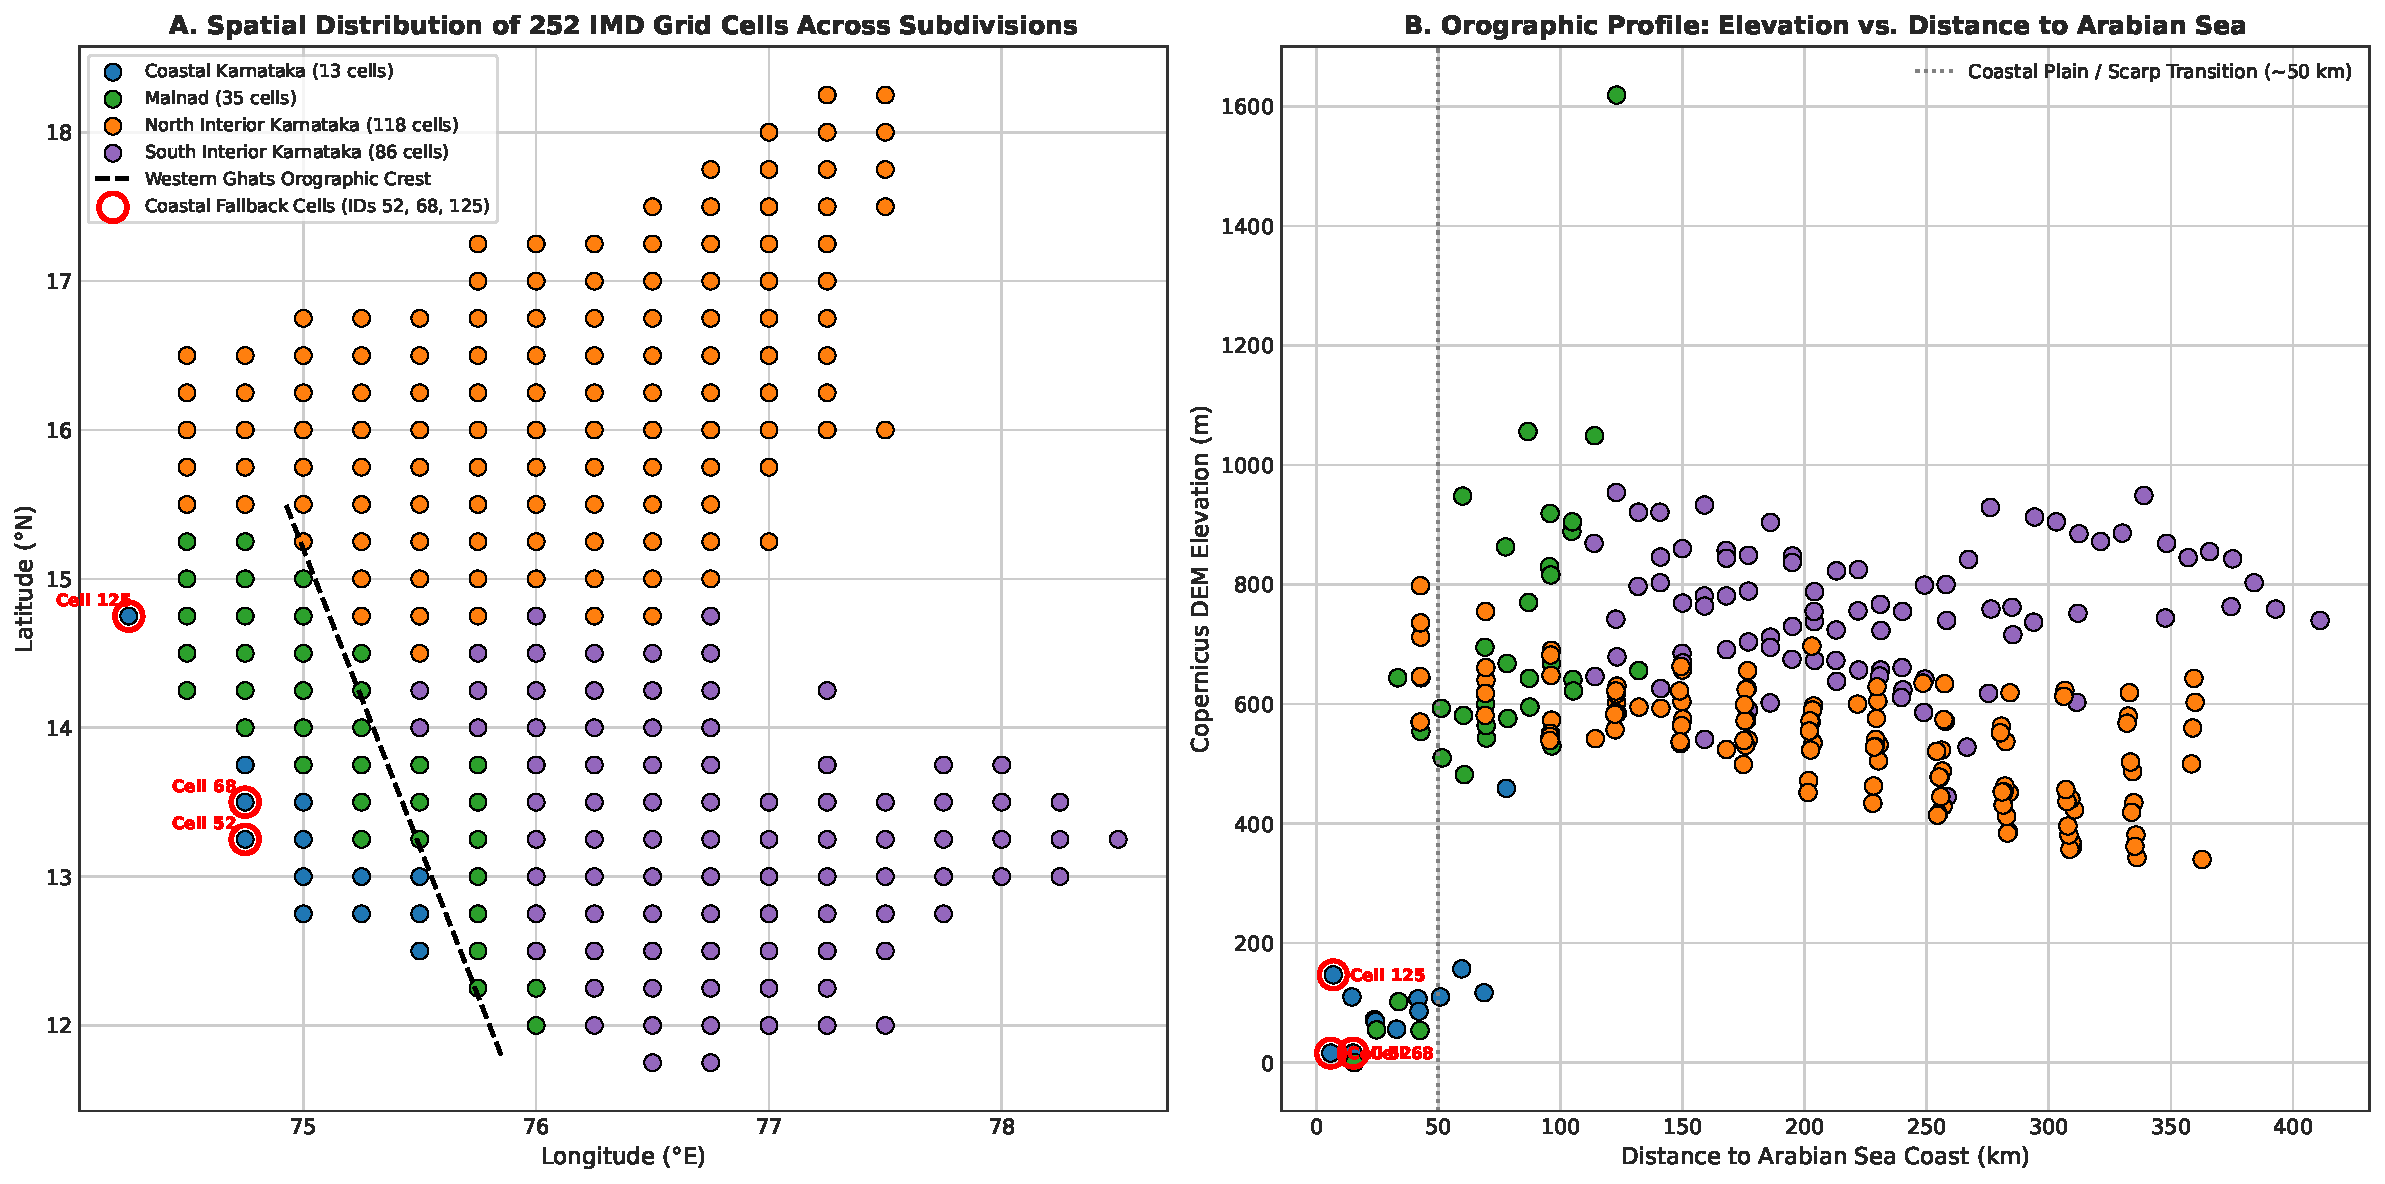
\includegraphics[width=0.82\textwidth]{figures/figure1_study_area}
\caption{High-resolution physiographic map of Karnataka depicting Copernicus GLO-90 DEM elevation, Western Ghats crest line, 252 IMD 0.25$^\circ$ gridded cells color-coded by meteorological subdivision, and the 3 coastal fallback cells (IDs 52, 68, 125).}
\label{fig:study_area}
\end{figure}

\subsection{Observational Target: IMD Gridded Rainfall}
The ground-truth observational target is the daily 0.25$^\circ \times 0.25^\circ$ ($\sim$27.75~km) gridded precipitation product developed by the National Climate Centre, India Meteorological Department (IMD), Pune \cite{pai2014}. The IMD gridded product is constructed via modified Shepard's inverse distance weighting interpolation from 6,955 quality-controlled surface rain gauges across the country \cite{rajeevan2006}. Each daily value represents the 24-hour accumulated rainfall ending at 08:30 Indian Standard Time (IST; corresponding to 03:00 UTC). We extract all 252 in-state terrestrial grid cells across the 2,556 calendar days spanning 1 January 2019 to 31 December 2025, yielding a full statewide dataset of $N = 640,836$ grid-cell-day observations.

\subsection{Reanalysis Features: ECMWF ERA5-Land}
Atmospheric thermodynamic state variables and surface energy/water fluxes are obtained from the ECMWF ERA5-Land reanalysis archive at 0.1$^\circ$ ($\sim$9~km) native hourly resolution across the complete 7-year span \cite{munoz2021}. Predictors extracted per grid cell include total precipitation (\texttt{tp}), surface runoff (\texttt{sro}), sub-surface total runoff (\texttt{ro}), 2-meter air temperature (\texttt{t2m}), 2-meter dewpoint temperature (\texttt{d2m}), surface pressure (\texttt{sp}), 10-meter eastward and northward wind components (\texttt{u10}, \texttt{v10}), surface solar radiation downwards (\texttt{ssrd}), surface thermal radiation downwards (\texttt{strd}), surface latent heat flux (\texttt{slhf}), surface sensible heat flux (\texttt{sshf}), total evaporation (\texttt{e}), potential evaporation (\texttt{pev}), skin reservoir water storage (\texttt{src}), volumetric soil water content across three layers (\texttt{swvl1}: 0--7~cm, \texttt{swvl2}: 7--28~cm, \texttt{swvl3}: 28--100~cm), and forecast albedo (\texttt{fal}).

\subsection{Static Orography, Topography, and Coastal Proximity}
Topographic elevation and terrain slope were computed from the Copernicus GLO-90 Digital Elevation Model (DEM) at 90-meter native spatial resolution \cite{copernicus2020}. For each IMD 0.25$^\circ$ grid cell centroid, we compute the local mean elevation (\texttt{elevation\_dem\_m}), the macro-scale topographic slope gradient in degrees (\texttt{slope\_dem\_deg}), the shortest Euclidean distance to the Arabian Sea coastline (\texttt{dist\_to\_coast\_km}), and the orthogonal distance to the Western Ghats mountain divide line (\texttt{dist\_to\_ghats\_crest\_km}).

\subsection{ERA5-Land De-accumulation Physics and Temporal Alignment}
In raw ECMWF ERA5-Land NetCDF archives, surface flux variables are stored as running integrals that reset to zero at 00:00 UTC each day. To recover hourly physical increments, backward differencing is performed:
\begin{align}
\Delta x_{t, 1} &= x_{t, 1} \quad \text{at 01:00 UTC} \\
\Delta x_{t, h} &= x_{t, h} - x_{t, h-1} \quad \text{for } h \in \{2, 3, \dots, 24\}
\end{align}
Across the statewide reanalysis archive evaluated across 2,543 calendar days (15 January 2019 to 31 December 2025, excluding the 14-day warm-up period), backward differencing was evaluated across 221,798,424 valid hourly forecast increments. Exactly 1,136,648 increments ($0.5125\%$) fell below the numerical check threshold of $\Delta x_h < -1.0 \times 10^{-5}$\;mm with a median magnitude of $-1.49 \times 10^{-5}$\;mm. These were confirmed as IEEE 754 single-precision floating-point rounding artifacts and clipped to zero via $\max(x, 0.0)$ to enforce non-negative mass conservation.

To establish the benchmark unlagged reanalysis total precipitation ($X_t^{\text{IMD}}$), hourly increments are integrated across the identical 24-hour IMD observation window (04:00 UTC on day $t-1$ through 03:00 UTC on day $t$):
\begin{equation}
X_t^{\text{IMD}} = \sum_{h=4}^{24} \Delta x_{t-1, h} + \sum_{h=1}^3 \Delta x_{t, h}
\end{equation}

\noindent \textbf{Strict Causal Latency Gating:} In our retrospective machine-learning pipeline, the hindcast issue boundary is fixed at $T_{\text{issue}} = \text{03:00 UTC on day } t-1$. All machine-learning predictors are strictly restricted to information available at or before $T_{\text{issue}}$. Consequently, the dynamic reanalysis feature is lagged by one full 24-hour cycle ($\text{era5\_tp\_lag\_1d} = X_{t-1}^{\text{IMD}}$), covering 04:00 UTC day $t-2$ to 03:00 UTC day $t-1$. All rolling aggregations apply an explicit one-step shift (\texttt{.shift(1)}), guaranteeing verified retrospective temporal separation with zero temporal leakage into the target accumulation period (Fig.~\ref{fig:methodology}).

\begin{figure}[htbp]
\centering
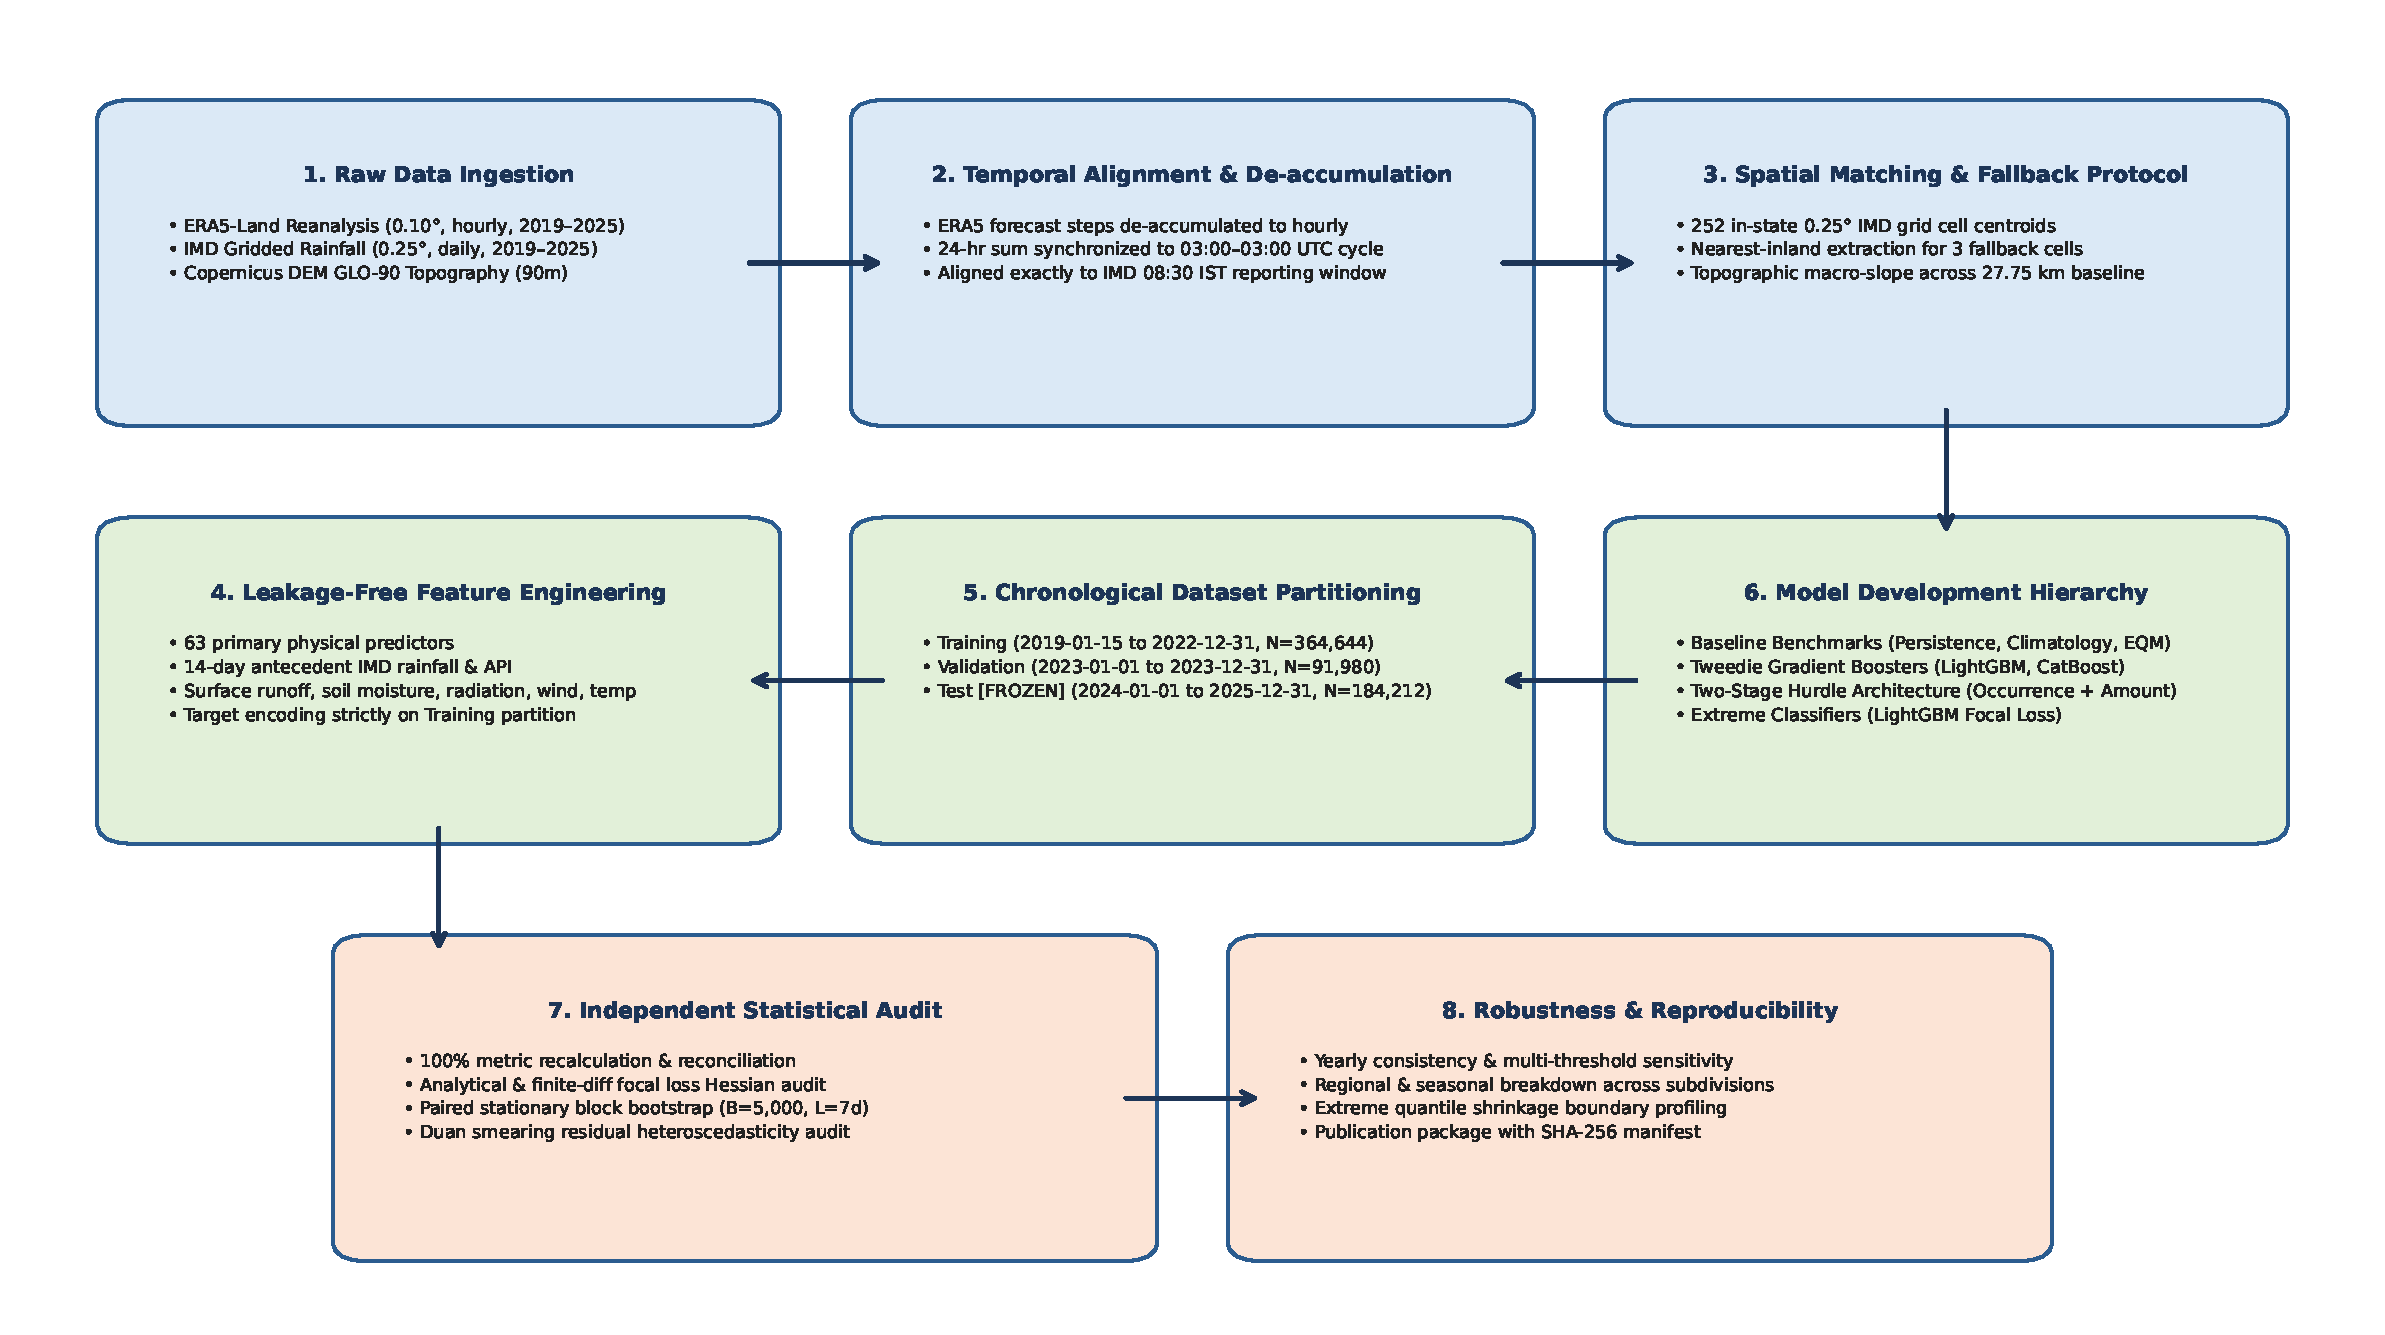
\includegraphics[width=0.88\textwidth]{figures/figure2_methodology}
\caption{End-to-end retrospective machine learning architecture depicting ERA5-Land flux de-accumulation, IMD gauge preparation, 24-h causal lag alignment, 63 primary feature engineering, temporal partitioning, model training, and multi-criteria evaluation.}
\label{fig:methodology}
\end{figure}

\subsection{Chronological Partitioning and Climatological Characteristics}
To respect temporal autocorrelation and evaluate out-of-sample forward generalization, the dataset is partitioned chronologically (Table~\ref{tab:dataset}):
\begin{itemize}
    \item \textbf{Training Partition (2019--2022):} 1,447 calendar days ($N = 364,644$ grid-cell days); mean daily rainfall = $3.7388$\;mm/day, std = $11.0264$\;mm, wet day frequency ($>0.1$\;mm) = $36.95\%$.
    \item \textbf{Validation Partition (2023):} 365 calendar days ($N = 91,980$ grid-cell days); marked by severe regional drought during the 2023 Southwest Monsoon: mean = $2.3571$\;mm/day vs. $3.7388$\;mm/day in training, wet day frequency = $27.39\%$. All model hyperparameters and classification thresholds were tuned strictly on this validation set.
    \item \textbf{Frozen Forward Test Partition (2024--2025):} 731 calendar days ($N = 184,212$ grid-cell days); mean = $3.5085$\;mm/day, std = $11.0006$\;mm, wet day frequency = $35.04\%$. This partition remained completely untouched until final benchmark scoring.
\end{itemize}

\begin{table}[htbp]
\centering
\caption{Temporal Dataset Partitioning and Climatological Characteristics (2019--2025)}
\label{tab:dataset}
\resizebox{\textwidth}{!}{
\begin{tabular}{p{2.5cm}p{3cm}p{2.2cm}p{3cm}p{2.5cm}p{2.2cm}r r r r r}
\toprule
\textbf{Data Source} & \textbf{Provider} & \textbf{Spatial Resolution} & \textbf{Temporal Resolution} & \textbf{Spatial Coverage} & \textbf{Temporal Span} & \textbf{Total Grid Cells} & \textbf{Total Records} & \textbf{Training Records} & \textbf{Validation Records} & \textbf{Test Records} \\
\midrule
IMD Gridded Daily Rainfall (Target) & India Meteorological Department (National Climate Centre, Pune) & 0.25$^\circ$ $\times$ 0.25$^\circ$ (~27.75 km) & Daily accumulation (03:00 UTC Day d-1 to 03:00 UTC Day d / 08:30 IST) & Karnataka State (252 in-state land cells, Lat 11.75$^\circ$N--18.50$^\circ$N, Lon 74.25$^\circ$E--78.50$^\circ$E) & 2019-01-01 to 2025-12-31 (7 calendar years, 2,557 days) & 252 & 640836 & 364,644 (2019-01-15 to 2022-12-31, 1,447 days; 14-day lag warmup buffer excluded) & 91,980 (2023-01-01 to 2023-12-31, 365 days; validation partition) & 184,212 (2024-01-01 to 2025-12-31, 731 days; 366d in 2024 leap year + 365d in 2025) \\
ERA5-Land Global Atmospheric Reanalysis (Predictors) & ECMWF / Copernicus Climate Change Service (C3S) & 0.10$^\circ$ $\times$ 0.10$^\circ$ (~9 km) aggregated to IMD 0.25$^\circ$ centroids & Hourly raw, de-accumulated and temporally aligned to IMD 03:00--03:00 UTC cycle & Karnataka state domain plus coastal maritime fallback buffer & 2019-01-01 to 2025-12-31 (84 monthly NetCDF files) & 252 & 640836 & 364,644 (Zero missing or infinite values across all 63 primary features) & 91,980 (Zero missing values; strictly out-of-sample temporal holdout) & 184,212 (Zero missing values; frozen out-of-sample temporal evaluation) \\
Copernicus GLO-90 Digital Elevation Model (Terrain) & European Space Agency (ESA) Copernicus Programme & 90 m native resolution, resampled to 0.25$^\circ$ grid centroids and macro-gradient slope & Static topographic surface & Centroid point elevation (m) and 27.75 km baseline macro-slope (degrees) & Static baseline & 252 & 252 & Identical static properties across all 252 IMD grid cells & Identical static properties across all 252 IMD grid cells & Identical static properties across all 252 IMD grid cells \\
\bottomrule
\end{tabular}
}
\end{table}

\subsection{Feature Matrix Architecture: The 63 Primary Predictors}
The finalized feature matrix contains exactly 63 numerical primary predictors ($X \in \mathbb{R}^{N \times 63}$) respecting the 24-hour causal latency boundary ($T_{\text{issue}} = \text{03:00 UTC on day } t-1$), organized into seven physical and hydrometeorological domains (Table~\ref{tab:features}):
\begin{enumerate}
    \item \textbf{Antecedent IMD Rainfall Memory (13 features):} Gauge lags ($y_{t-1}, y_{t-2}, y_{t-3}, y_{t-7}, y_{t-14}$), rolling sums (3d, 7d, 14d), rolling means (3d, 7d, 14d), 7-day rolling maximum, and the 14-day Antecedent Precipitation Index ($\text{API}_{14} = \sum_{k=1}^{14} 0.85^k y_{t-k}$).
    \item \textbf{ERA5-Land Precipitation \& Hydrological Balance (14 features):} Reanalysis total precipitation lags and rolling sums, surface runoff (\texttt{sro\_lag\_1d}), sub-surface total runoff (\texttt{ro\_lag\_1d}), skin reservoir storage (\texttt{src\_lag\_1d}), evaporation components (\texttt{e}, \texttt{pev}, \texttt{evabs}, \texttt{evatc}, \texttt{evavt}), and albedo (\texttt{fal}).
    \item \textbf{Atmospheric Thermodynamic State \& Wind (12 features):} 2-meter temperature metrics (\texttt{mean}, \texttt{min}, \texttt{max}, diurnal range), 2-meter dewpoint temperature, dewpoint depression ($\Delta T_d = T - T_d$), surface pressure, and 10-meter wind speed metrics.
    \item \textbf{Soil Moisture Profiles \& Energy Fluxes (9 features):} Volumetric soil water across three soil layers (\texttt{swvl1}, \texttt{swvl2}, \texttt{swvl3}), downward shortwave and longwave radiation fluxes (\texttt{ssrd}, \texttt{strd}), and sensible and latent turbulent heat fluxes (\texttt{sshf}, \texttt{slhf}).
    \item \textbf{Topography, Elevation \& Coastal Proximity (6 features):} GLO-90 DEM elevation, terrain slope, distance to coast, distance to Western Ghats crest, and grid centroid coordinates.
    \item \textbf{Cyclic Temporal Ephemeris (7 features):} Calendar month, Julian day of year, harmonic trigonometric transformations ($\sin, \cos$ of day of year and month), and monsoon seasonal indicator.
    \item \textbf{Regional Categorical Encodings (2 features):} Meteorological subdivision and agro-climatic zone ID, target mean-encoded strictly on the 2019--2022 training partition.
\end{enumerate}

\begin{table}[htbp]
\centering
\caption{Input Feature Groups, Predictor Schema, and Pipeline Causal Gating (63 Primary Features)}
\label{tab:features}
\resizebox{\textwidth}{!}{
\begin{tabular}{p{3.5cm}cp{5.5cm}p{4cm}p{5.5cm}}
\toprule
\textbf{Feature Group} & \textbf{Predictor Count} & \textbf{Representative Variables} & \textbf{Temporal Alignment} & \textbf{Scientific Relevance} \\
\midrule
1. Antecedent IMD Rainfall Memory & 13 & target\_rain\_lag\_1d, lag\_2d, lag\_3d, lag\_7d, lag\_14d, roll\_3d\_sum, roll\_7d\_sum, roll\_14d\_sum, roll\_3d\_mean, roll\_7d\_mean, roll\_14d\_mean, roll\_7d\_max, api\_14d & 03:00 UTC Day d-1 (Lag 1) to Day d-14 (all shifted strictly by $\ge$1 day) & Ground-truth antecedent precipitation persistence, catchment moisture memory, and 14-day antecedent precipitation index (decay k=0.85). \\
2. ERA5-Land Precipitation \& Hydrological Balance & 14 & era5\_tp\_lag\_1d, lag\_2d, lag\_3d, roll\_3d\_sum, roll\_7d\_sum, ro\_lag\_1d (total runoff), sro\_lag\_1d (surface runoff), src\_lag\_1d (skin reservoir), e\_lag\_1d, pev\_lag\_1d, evabs\_lag\_1d, evatc\_lag\_1d, evavt\_lag\_1d, fal\_lag\_1d & De-accumulated daily sum 04:00 UTC Day d-2 to 03:00 UTC Day d-1 (Lag 1) & Antecedent reanalysis-derived precipitation and land-surface flux memory, model-derived runoff proxies of soil saturation, canopy interception storage, and evapotranspiration demand. \\
3. Atmospheric Thermodynamic State \& Wind & 12 & t2m\_mean\_lag\_1d, t2m\_min\_lag\_1d, t2m\_max\_lag\_1d, temp\_range\_lag\_1d, d2m\_mean\_lag\_1d, dewpoint\_depression\_lag\_1d, t2m\_roll\_3d\_mean, t2m\_roll\_7d\_mean, sp\_lag\_1d, wind\_speed\_lag\_1d, wind\_roll\_3d\_mean, wind\_roll\_7d\_mean & Daily mean, min, max over 24-hr cycle ending 03:00 UTC Day d-1 & Boundary-layer thermal structure, moisture saturation deficit (sub-cloud relative humidity proxy), synoptic surface pressure, and near-surface 10-meter wind speed circulation conditions. \\
4. Soil Moisture Profiles \& Radiative/Turbulent Fluxes & 9 & swvl1\_lag\_1d (0-7 cm), swvl1\_lag\_3d, swvl1\_lag\_7d, swvl2\_lag\_1d (7-28 cm), swvl3\_lag\_1d (28-100 cm), ssrd\_lag\_1d (solar), strd\_lag\_1d (thermal), slhf\_lag\_1d (latent), sshf\_lag\_1d (sensible) & Layer volumetric water content and daily accumulated radiative/turbulent energy fluxes ending 03:00 UTC Day d-1 & Root-zone soil water storage, cloud-cover radiative trapping (downward longwave), clear-sky solar insolation, and surface sensible/latent heat partitioning. \\
5. Topography, Elevation \& Spatial Proximity & 6 & elevation\_dem\_m, slope\_dem\_deg, latitude, longitude, dist\_to\_coast\_km, dist\_to\_ghats\_crest\_km & Static spatial coordinates and Copernicus DEM GLO-90 terrain metrics & Orographic uplift forcing along the Western Ghats barrier, maritime-continental continentality gradient, and regional terrain slope gradient. \\
6. Temporal Ephemeris \& Astronomical Cycles & 7 & month, day\_of\_year, sin\_day\_of\_year, cos\_day\_of\_year, sin\_month, cos\_month, is\_monsoon & Harmonic cyclical transformation of Julian date and calendar indicators known at issue time & Synoptic seasonal climatology, solar declination angle, and Southwest Monsoon boundary definition. \\
7. Primary Categorical Regional Predictors & 2 & subdivision (Coastal Karnataka, Malnad, North Interior, South Interior), zone\_id (10 agroclimatic zones) [target-encoded into subdivision\_enc, zone\_id\_enc] & Static administrative / agroclimatic classification (target encoding fitted strictly on Training partition) & Regional agroclimatic baselines and spatial climatological stratification. \\
Auxiliary Quality Flag (Separate from Primary Predictors) & 1 & is\_coastal\_fallback (binary 0/1 indicator for Grid-Cell IDs 52, 68, 125) & Static data-quality indicator & Flags coastal cells touching ocean boundaries requiring nearest-land neighbor fallback extraction. \\
\bottomrule
\end{tabular}
}
\end{table}

\subsection{Model Formulations Across Structural Tiers}
We formulate and evaluate 11 predictive models spanning five structural tiers:
\begin{itemize}
    \item \textbf{Tier 0 (Naive Baselines):} Autoregressive Persistence ($y_t = y_{t-1}$) and Day-of-Year (DOY) Climatology (historical calendar-day mean per grid cell).
    \item \textbf{Tier 1 (Raw Reanalysis Benchmark):} Uncalibrated antecedent ERA5-Land precipitation ($X_{t-1}^{\text{IMD}}$).
    \item \textbf{Tier 2 (Statistical Downscaling):} Empirical Quantile Mapping (EQM) \cite{piani2011} fitted with 100 empirical quantile knots per IMD cell on the 2019--2022 training partition.
    \item \textbf{Tier 3 (Regularized Linear Baselines):} L2-regularized Ridge Regression ($\alpha = 100.0$) and ElasticNet Regression ($\alpha = 0.1$, $\text{l1\_ratio} = 0.5$) fitted on standardized predictors.
    \item \textbf{Tier 4 (Machine Learning Regressors):} 
    \begin{itemize}
        \item \textbf{LightGBM Tweedie ($p=1.5$):} GBDT optimizing Compound Poisson-Gamma deviance with log link \cite{ke2017}.
        \item \textbf{CatBoost Tweedie ($p=1.5$):} Symmetric oblivious decision trees optimizing Tweedie deviance \cite{prokhorenkova2018}.
        \item \textbf{LightGBM Log-Ordinary with Duan Smearing:} Log-transformed target regressor adjusted with Duan's non-parametric smearing factor \cite{duan1983}:
        \begin{equation}
        \hat{y}_t = \exp(\hat{\mu}_t) \cdot \frac{1}{N} \sum_{i=1}^N \exp(e_i)
        \end{equation}
        \item \textbf{Two-Stage Hurdle Expected Value:} Stage 1 binary logistic classifier predicting rain occurrence ($p_t = P(y_t > 0)$) coupled with Stage 2 LightGBM Gamma regression predicting positive rainfall ($\mu_t^+$), combined as $\hat{y}_t = p_t \cdot \mu_t^+$ \cite{cragg1971}.
    \end{itemize}
\end{itemize}

\subsection{Dedicated Heavy Rainfall Classification: Custom Asymmetric Focal Loss}
Because heavy rainfall events ($\ge 64.5$\;mm/day) account for only $0.6878\%$ of test records, standard binary cross-entropy exhibits extreme miss rates. We implement a custom Lin et al. \cite{lin2017} Focal Loss objective in LightGBM:
\begin{equation}
\text{FL}(p_t) = -\alpha_t (1 - p_t)^\gamma \log(p_t)
\end{equation}
where $\gamma = 2.0$ is the focusing parameter and $\alpha = 0.75$ balances positive-class prevalence. The first and second custom analytical gradients with respect to raw logit margin $z$ are:
\begin{align}
g_1 &= \frac{\partial \text{FL}}{\partial z} = \begin{cases}
-\alpha (1 - p)^\gamma [1 - \gamma p \log p - p] & \text{if } y = 1 \\
(1 - \alpha) p^\gamma [p - \gamma (1 - p) \log(1 - p)] & \text{if } y = 0
\end{cases} \\
h_1 &= \frac{\partial^2 \text{FL}}{\partial z^2} \approx \max\left( \frac{\partial g_1}{\partial z}, 10^{-6} \right)
\end{align}
The optimal decision threshold $p^* = 0.53$ was selected strictly on the 2023 validation set to maximize the Critical Success Index (CSI).

\subsection{Evaluation Metrics and Paired Stationary Block Bootstrapping}
Continuous performance is evaluated using Root Mean Squared Error (RMSE), Mean Absolute Error (MAE), Mean Bias, Percentage Bias (PBias), Pearson correlation coefficient ($r$), Nash-Sutcliffe Efficiency (NSE) \cite{nash1970}, Classic Kling-Gupta Efficiency (KGE-2009) \cite{gupta2009}, and Modified Kling-Gupta Efficiency (KGE-2012) \cite{kling2012}:
\begin{equation}
\text{KGE-2012} = 1 - \sqrt{(r - 1)^2 + (\beta - 1)^2 + (\gamma - 1)^2}
\end{equation}
where $\beta = \mu_{\text{pred}} / \mu_{\text{obs}}$ and $\gamma = \text{CV}_{\text{pred}} / \text{CV}_{\text{obs}}$. Categorical heavy-rain alerting is scored via Probability of Detection (POD / Recall), False Alarm Ratio (FAR), Precision, Critical Success Index ($\text{CSI} = H / (H + M + F)$), and Heidke Skill Score (HSS).

To account for strong spatial cross-correlation across 252 grid cells and temporal autocorrelation across consecutive days, statistical significance is verified via stationary paired block bootstrapping \cite{kunsch1989, politis1994}. Resampling is performed across entire statewide calendar days with $B = 2,000$ iterations under block lengths of $L = 7\text{ days}$ (synoptic scale) and $L = 14\text{ days}$ (intraseasonal scale).

\newpage
\section{Results and Discussions}

\subsection{Continuous Daily Rainfall Estimation and Multi-Criteria Benchmarking}
Table~\ref{tab:benchmarking} details out-of-sample forward evaluation on the frozen 2024--2025 test partition ($N = 184,212$ instances). Rather than exhibiting a single universally superior architecture, the top three machine-learning models establish distinct multi-criteria trade-offs:
\begin{itemize}
    \item \textbf{Two-Stage Hurdle Expected Value} attains the lowest overall test RMSE ($7.4241$\;mm), highest Pearson correlation ($r = 0.7380$), and highest Nash-Sutcliffe Efficiency ($\text{NSE} = 0.5443$).
    \item \textbf{CatBoost Tweedie} achieves the highest Modified Kling-Gupta Efficiency ($\text{KGE-2012} = 0.6261$) alongside near-champion RMSE ($7.4335$\;mm).
    \item \textbf{LightGBM Tweedie} delivers the lowest Mean Absolute Error ($\text{MAE} = 2.8993$\;mm) and lowest mean bias ($-0.0179$\;mm, or $-0.51\%$ relative bias).
\end{itemize}

All three machine-learning architectures drastically outperform naive autoregressive Persistence ($\text{RMSE} = 10.3582$\;mm; $\sim$28.3\% error reduction), raw antecedent ERA5-Land reanalysis ($\text{RMSE} = 10.4550$\;mm; $\sim$28.9\% error reduction), and grid-cell-wise Empirical Quantile Mapping ($\text{EQM}$, $\text{RMSE} = 11.1970$\;mm, $\text{NSE} = -0.0366$) (Fig.~\ref{fig:hexbin} and Fig.~\ref{fig:benchmarking}).

\begin{table}[htbp]
\centering
\caption{Comprehensive Out-of-Sample Model Benchmarking Portfolio (Test Partition 2024--2025; $N = 184,212$)}
\label{tab:benchmarking}
\resizebox{\textwidth}{!}{
\begin{tabular}{lllr r r r r r r r r}
\toprule
\textbf{Model Hierarchy Tier} & \textbf{Model Name} & \textbf{Loss Objective} & \textbf{RMSE mm} & \textbf{MAE mm} & \textbf{Mean Bias mm} & \textbf{PBias pct} & \textbf{Pearson r} & \textbf{NSE} & \textbf{Classic KGE 2009} & \textbf{Modified KGE 2012} & \textbf{Heavy CSI 64.5mm} \\
\midrule
Tier 0 (Naive Baselines) & Rainfall Persistence & Zero Learning & 10.3582 & 3.7508 & 0.0 & 0.0 & 0.5565 & 0.1129 & 0.5565 & 0.5565 & 0.2361 \\
Tier 0 (Naive Baselines) & Grid-cell DOY Climatology & Zero Learning & 10.1155 & 4.3078 & 0.2296 & 6.54 & 0.4313 & 0.154 & 0.3068 & 0.2851 & 0.0144 \\
Tier 1 (Raw Reanalysis) & Antecedent ERA5-Land Total Precip & Zero Learning & 10.455 & 4.1416 & 0.556 & 15.85 & 0.4911 & 0.0963 & 0.451 & 0.4111 & 0.1233 \\
Tier 2 (Statistical Downscaling) & Empirical Quantile Mapping (EQM) & Non-Parametric Knots & 11.197 & 4.2117 & 0.3867 & 11.02 & 0.4941 & -0.0366 & 0.4818 & 0.4763 & 0.1969 \\
Tier 3 (Linear Baselines) & Ridge Regression & L2 Regularized Linear & 7.975 & 3.3905 & 0.3308 & 9.43 & 0.6894 & 0.4742 & 0.5613 & 0.5184 & 0.2299 \\
Tier 3 (Linear Baselines) & ElasticNet Regression & L1/L2 Regularized Linear & 8.0156 & 3.3999 & 0.3034 & 8.65 & 0.6853 & 0.4688 & 0.5496 & 0.5101 & 0.2211 \\
Tier 4 (Machine Learning) & LightGBM RMSE & RMSE (L2) & 7.4982 & 3.0806 & 0.2698 & 7.69 & 0.732 & 0.5352 & 0.619 & 0.5812 & 0.3016 \\
Tier 4 (Machine Learning) & LightGBM Log OrdinaryInverse & Log MSE & 7.8497 & 2.615 & -1.3274 & -37.83 & 0.726 & 0.4906 & 0.3703 & 0.5276 & 0.2271 \\
Tier 4 (Machine Learning) & LightGBM Log DuanSmearing & Log MSE & 7.5893 & 2.9488 & -0.2105 & -6.0 & 0.726 & 0.5238 & 0.6439 & 0.6722 & 0.3509 \\
Tier 4 (Machine Learning) & LightGBM Tweedie p1.5 & Compound Poisson-Gamma (p=1.5) & 7.4427 & 2.8993 & -0.0179 & -0.51 & 0.7363 & 0.542 & 0.6218 & 0.6245 & 0.2868 \\
Tier 4 (Machine Learning) & CatBoost Tweedie p1.5 & Compound Poisson-Gamma (p=1.5) & 7.4335 & 2.9186 & 0.0388 & 1.11 & 0.737 & 0.5431 & 0.6318 & 0.6261 & 0.3033 \\
Tier 4 (Machine Learning) & Hurdle ExpectedValue & Two-Stage Hurdle Expected Value & 7.4241 & 2.93 & 0.0342 & 0.97 & 0.738 & 0.5443 & 0.6165 & 0.6114 & 0.3072 \\
\bottomrule
\end{tabular}
}
\end{table}

\begin{figure}[htbp]
\centering
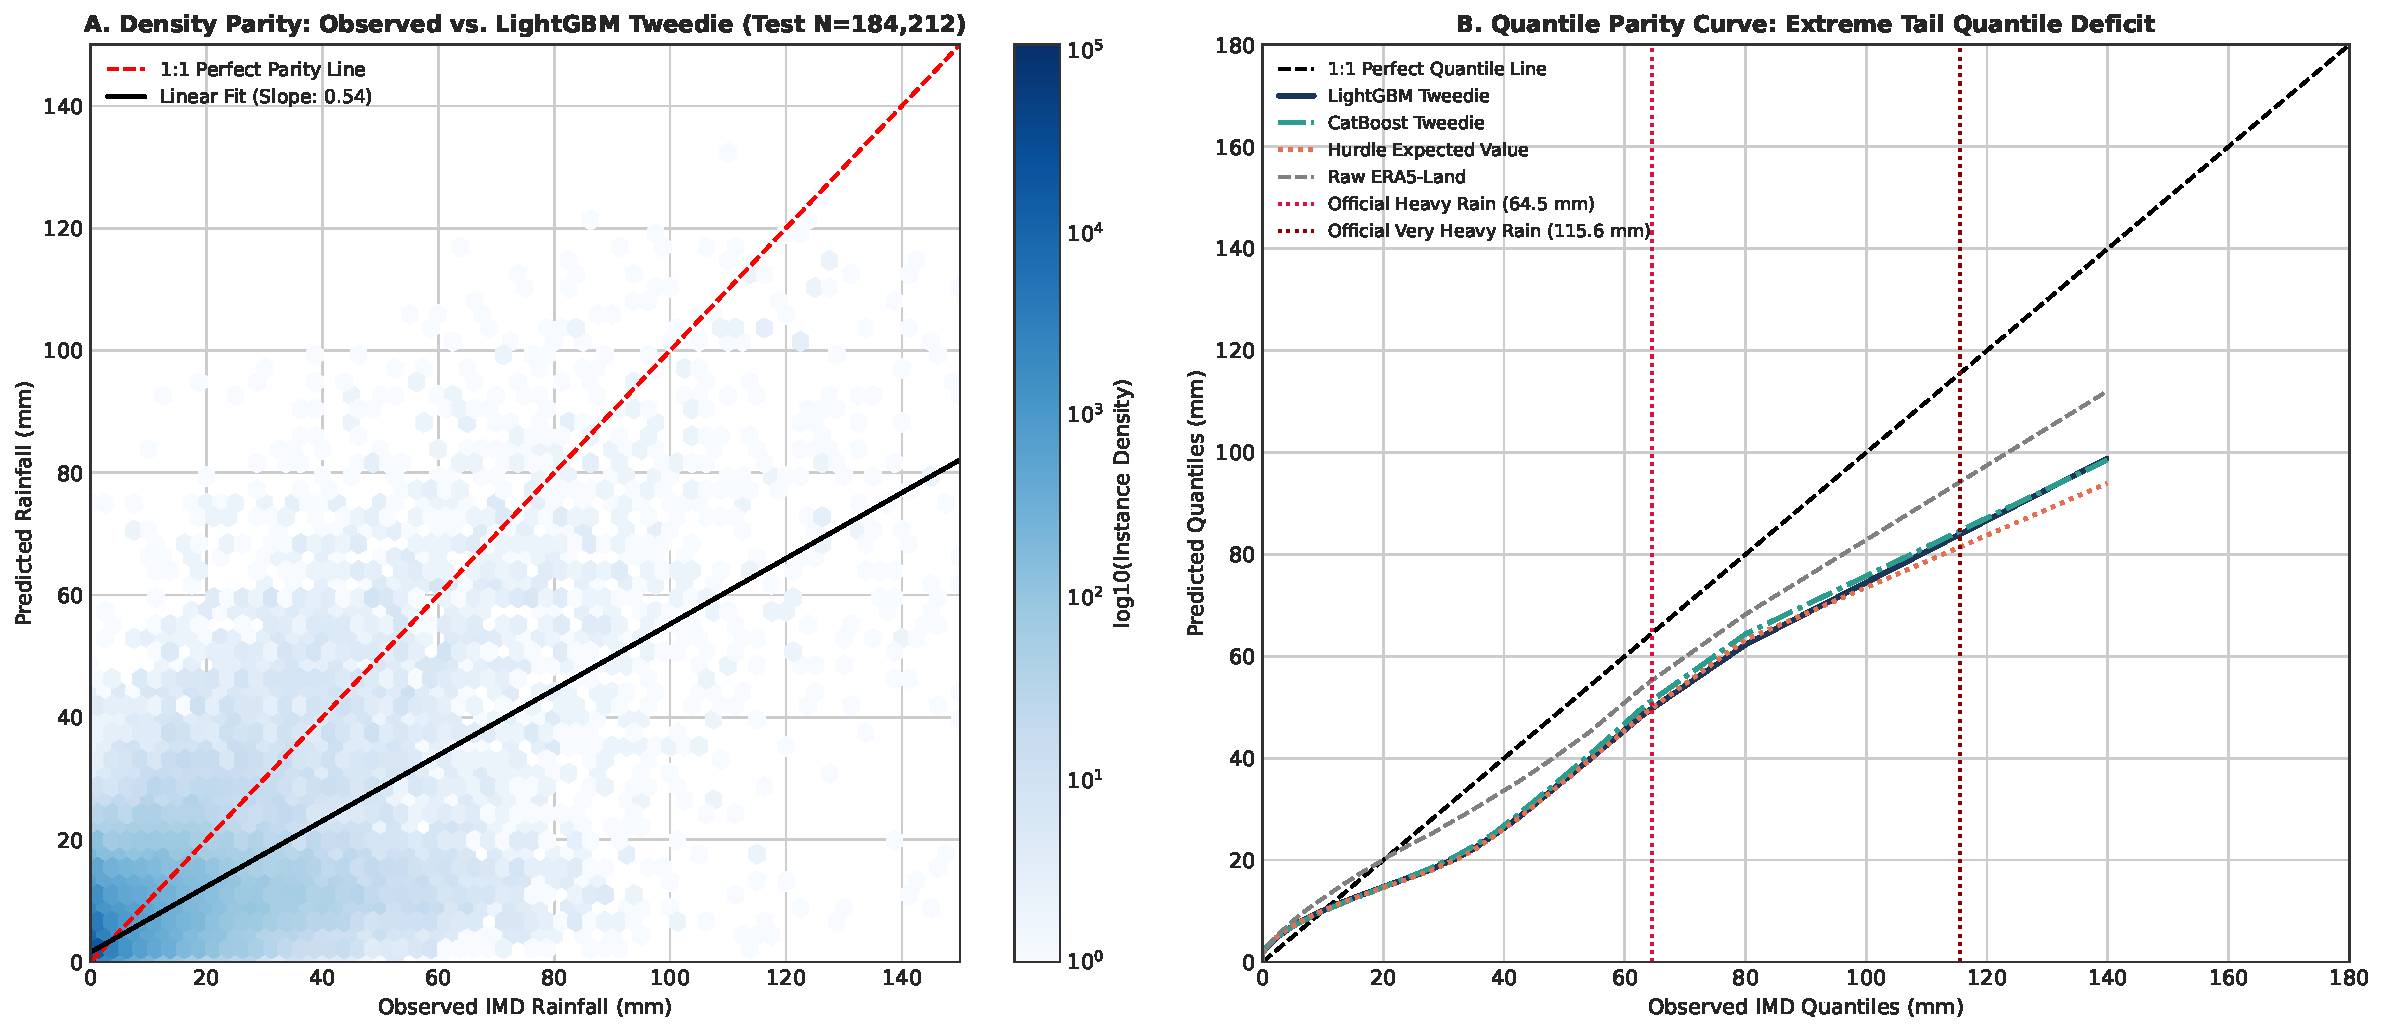
\includegraphics[width=0.72\textwidth]{figures/figure3_observed_predicted}
\caption{Density parity hexbin between observed and predicted daily rainfall on the 2024--2025 test partition. Color bar represents log-scaled instance density.}
\label{fig:hexbin}
\end{figure}

\begin{figure}[htbp]
\centering
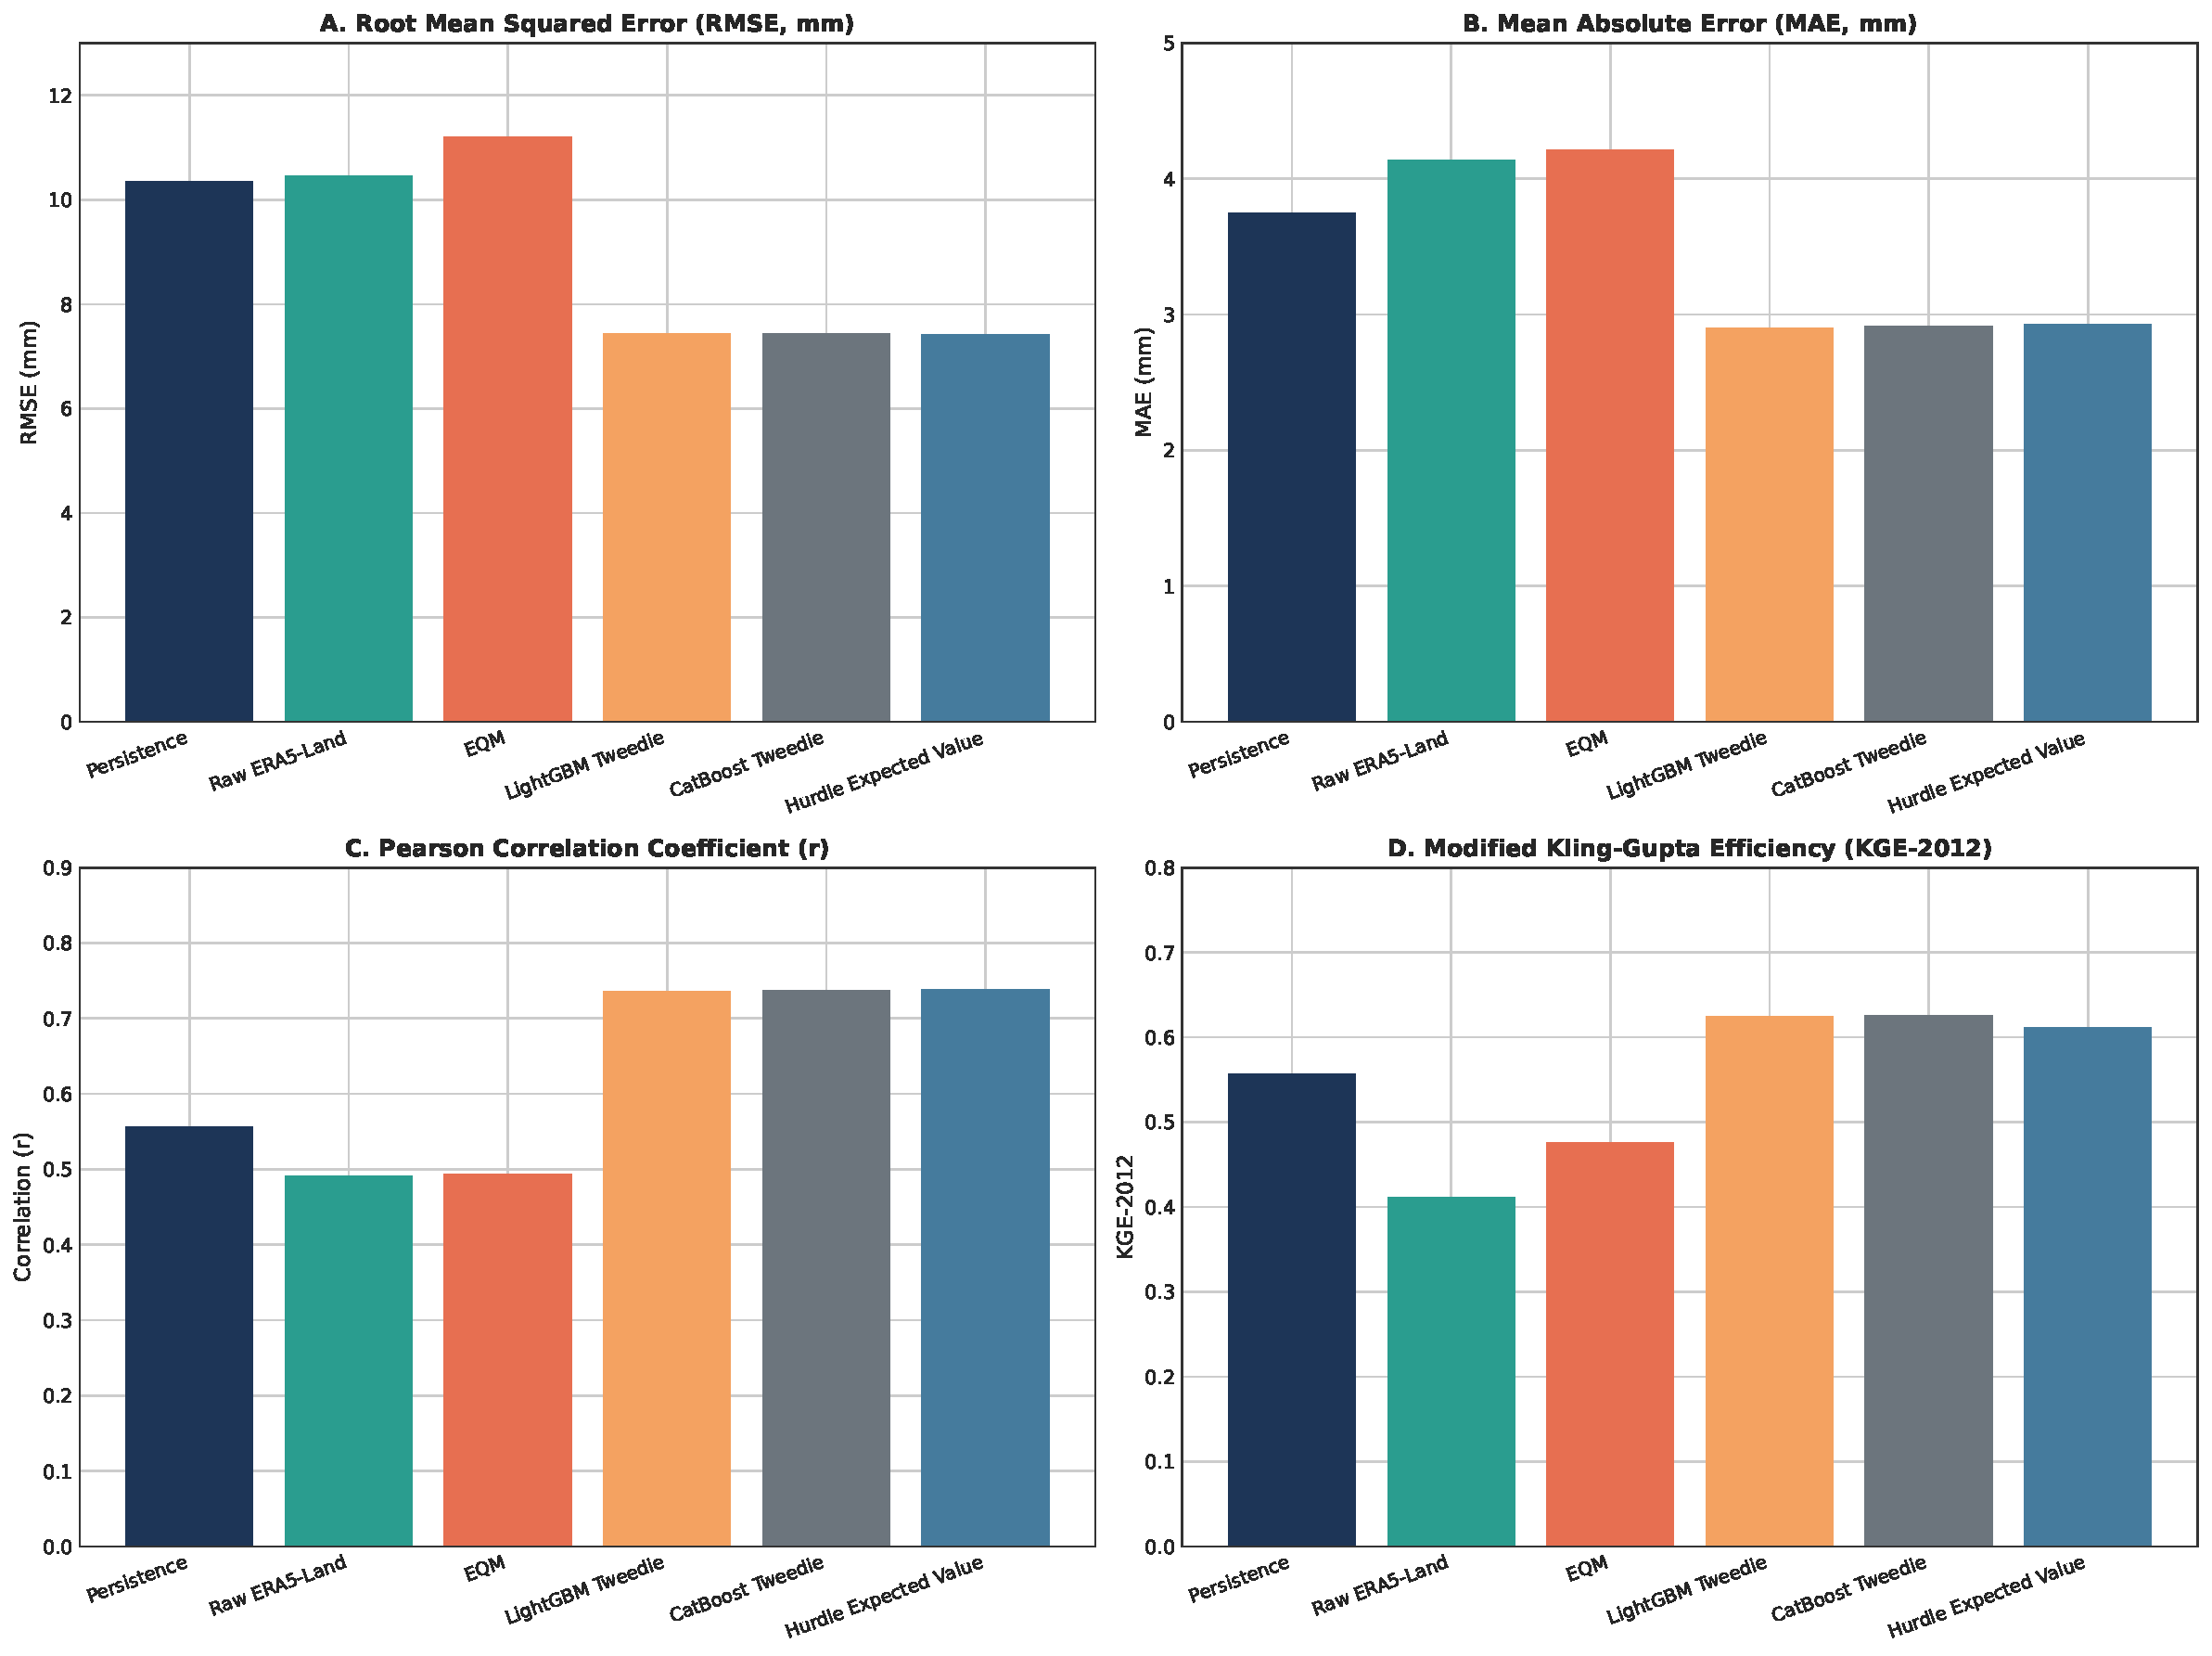
\includegraphics[width=0.88\textwidth]{figures/figure4_model_benchmarking}
\caption{Comparative bar panels showing RMSE, MAE, Pearson correlation, and KGE-2012 across all 11 evaluated models on the frozen test partition.}
\label{fig:benchmarking}
\end{figure}

\subsection{Dedicated Heavy Rainfall Detection and Retrospective Classifier Evaluation}
Table~\ref{tab:heavy_rain} presents contingency scoring for heavy precipitation events ($\ge 64.5$\;mm/day; 1,267 observed events out of 184,212 test instances; prevalence = $0.6878\%$).

\begin{table}[htbp]
\centering
\caption{Dedicated Heavy Rainfall ($\ge 64.5$\;mm) Contingency and Skill Score Evaluation (Test 2024--2025)}
\label{tab:heavy_rain}
\resizebox{\textwidth}{!}{
\begin{tabular}{llp{4.5cm}r r r r r r r r r r r}
\toprule
\textbf{Model Name} & \textbf{Decision Threshold} & \textbf{Threshold Selection Basis} & \textbf{Hits} & \textbf{Misses} & \textbf{False Alarms} & \textbf{Correct Negatives} & \textbf{Precision} & \textbf{POD Recall} & \textbf{FAR} & \textbf{CSI} & \textbf{HSS} & \textbf{ETS} & \textbf{PR AUC} \\
\midrule
LightGBM\_Heavy\_FocalLoss & 0.53 & Validation-selected decision threshold p*=0.53 chosen on 2023 Validation to maximize CSI & 595 & 672 & 427 & 182518 & 0.5822 & 0.4696 & 0.4178 & 0.3512 & 0.5169 & 0.3485 & 0.5084 \\
LightGBM\_Heavy\_ClassWeighted & 0.96 & Validation-selected decision threshold p*=0.96 chosen on 2023 Validation to maximize CSI & 688 & 579 & 722 & 182223 & 0.4879 & 0.543 & 0.5121 & 0.3459 & 0.5105 & 0.3427 & 0.4853 \\
CatBoost\_Heavy\_ClassWeighted & 0.98 & Validation-selected decision threshold p*=0.98 chosen on 2023 Validation to maximize CSI & 608 & 659 & 515 & 182430 & 0.5414 & 0.4799 & 0.4586 & 0.3412 & 0.5056 & 0.3383 & 0.4739 \\
Rainfall\_Persistence & 64.5 mm (fixed physical) & Physical 64.5 mm threshold applied directly to y\_{t-1} observations & 484 & 783 & 783 & 182162 & 0.382 & 0.382 & 0.618 & 0.2361 & 0.3777 & 0.2328 & nan \\
Raw\_ERA5\_Land & 64.5 mm (fixed physical) & Physical 64.5 mm threshold applied directly to raw antecedent total precipitation & 231 & 1036 & 606 & 182339 & 0.276 & 0.1823 & 0.724 & 0.1233 & 0.2153 & 0.1206 & nan \\
Empirical\_Quantile\_Mapping\_EQM & 64.5 mm (fixed physical) & Physical 64.5 mm threshold applied to grid-cell-specific quantile-mapped rainfall & 372 & 895 & 622 & 182323 & 0.3742 & 0.2936 & 0.6258 & 0.1969 & 0.325 & 0.194 & nan \\
\bottomrule
\end{tabular}
}
\end{table}

\begin{figure}[htbp]
\centering
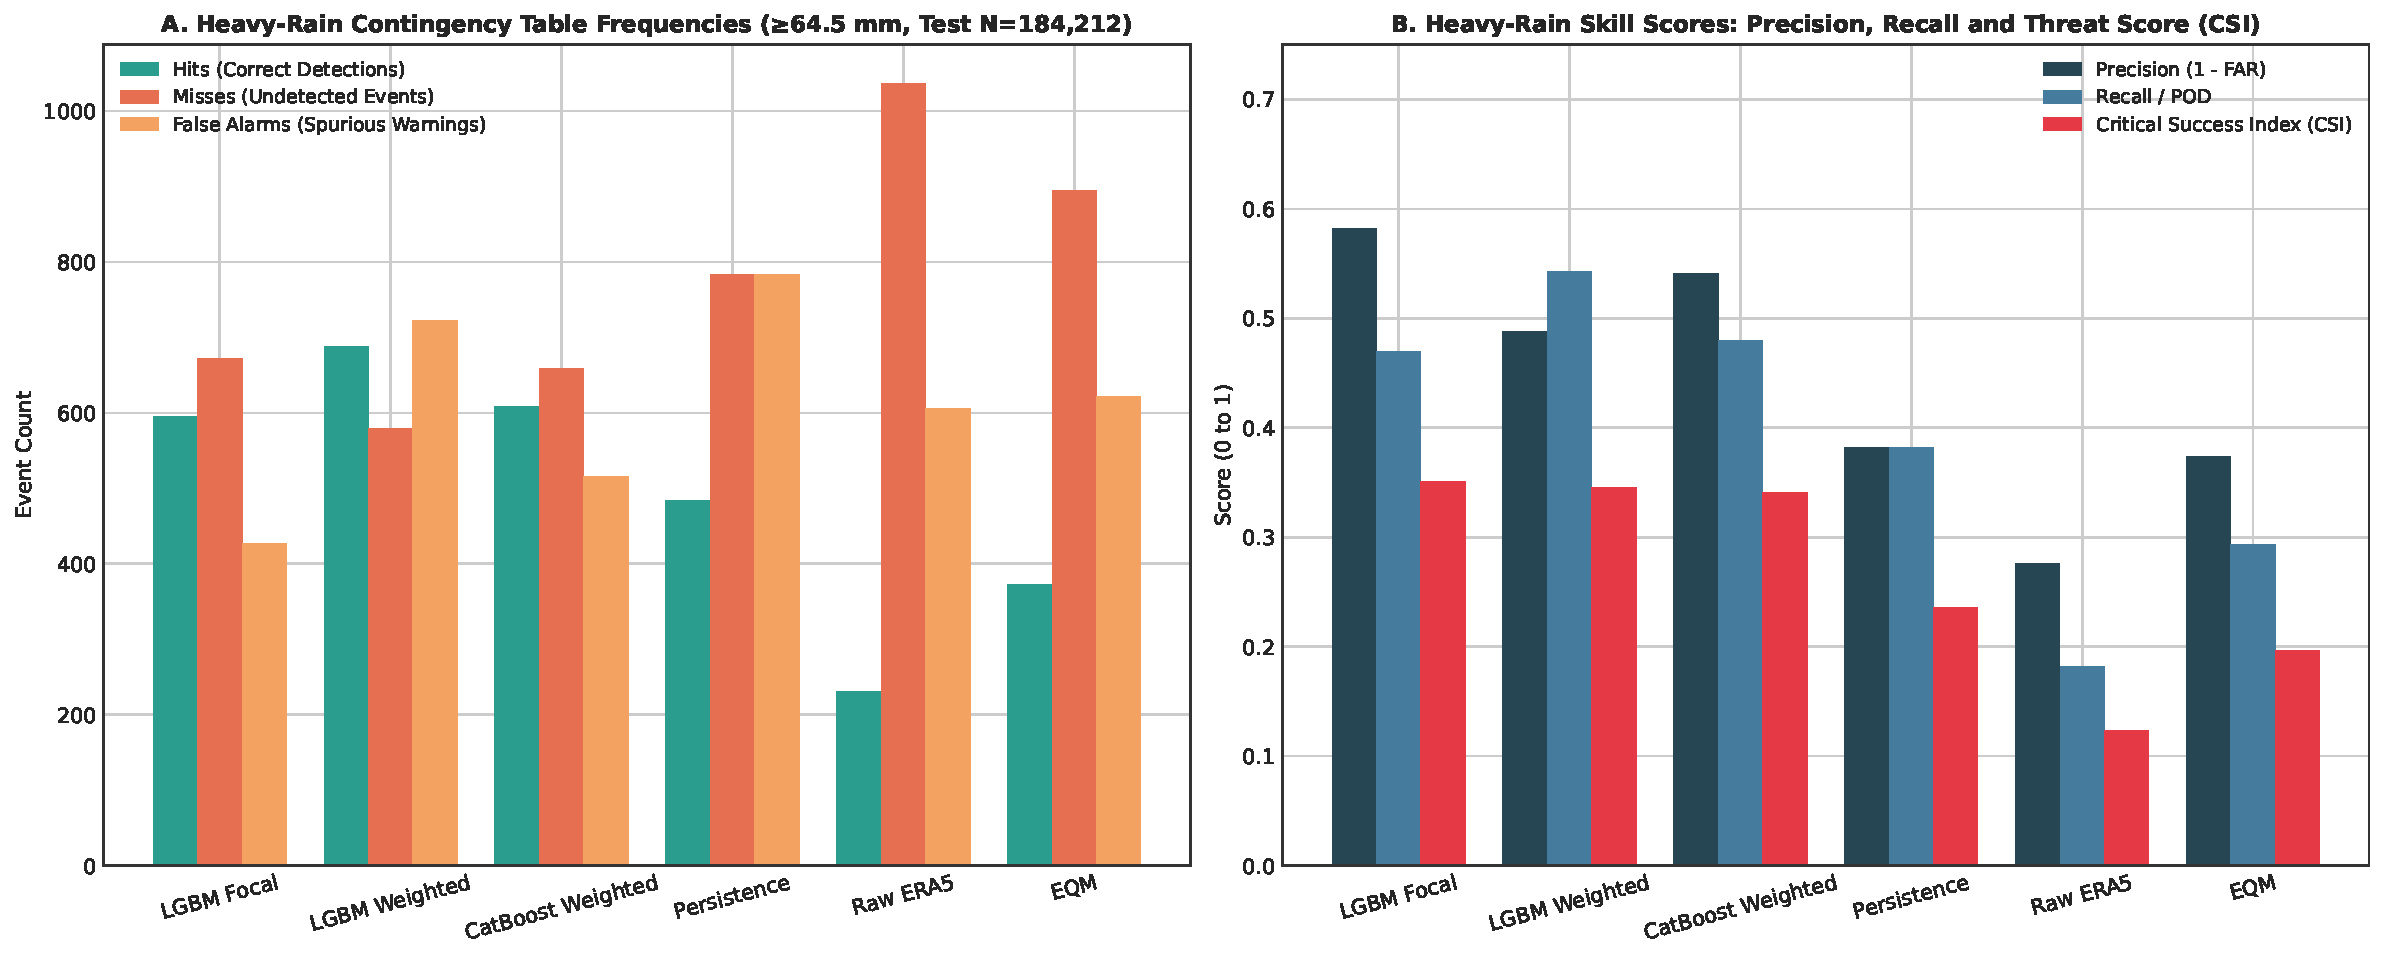
\includegraphics[width=0.85\textwidth]{figures/figure5_heavy_rain_detection}
\caption{Synoptic heavy-rain detection performance. Panel A shows contingency breakdown (Hits, Misses, False Alarms); Panel B shows Precision-Recall curves across classification architectures.}
\label{fig:heavy_rain}
\end{figure}

At the validation-selected decision threshold $p^* = 0.53$, the LightGBM Focal Loss classifier achieves a test Probability of Detection of $46.96\%$ ($595$ hits), Precision of $58.22\%$, Critical Success Index (CSI) of $0.3512$, and FAR of $41.78\%$ ($427$ false alarms), while missing $53.04\%$ of observed heavy events ($672$ misses) (Fig.~\ref{fig:heavy_rain}). In comparison, standard class-weighted LightGBM incurs $722$ false alarms ($\text{FAR} = 51.21\%$). Thus, Focal Loss achieves a $40.86\%$ reduction in false alarms while retaining superior precision and CSI. However, missing more than half of true extreme events demonstrates that this model represents an experimental retrospective classifier rather than an operational disaster-warning system.

\subsection{Feature Attribution: Tree Gain, Permutation, and Ablation Dynamics}
Figure~\ref{fig:attribution} and Table~\ref{tab:ablation} evaluate predictor importance across the 63 primary features.

\begin{figure}[htbp]
\centering
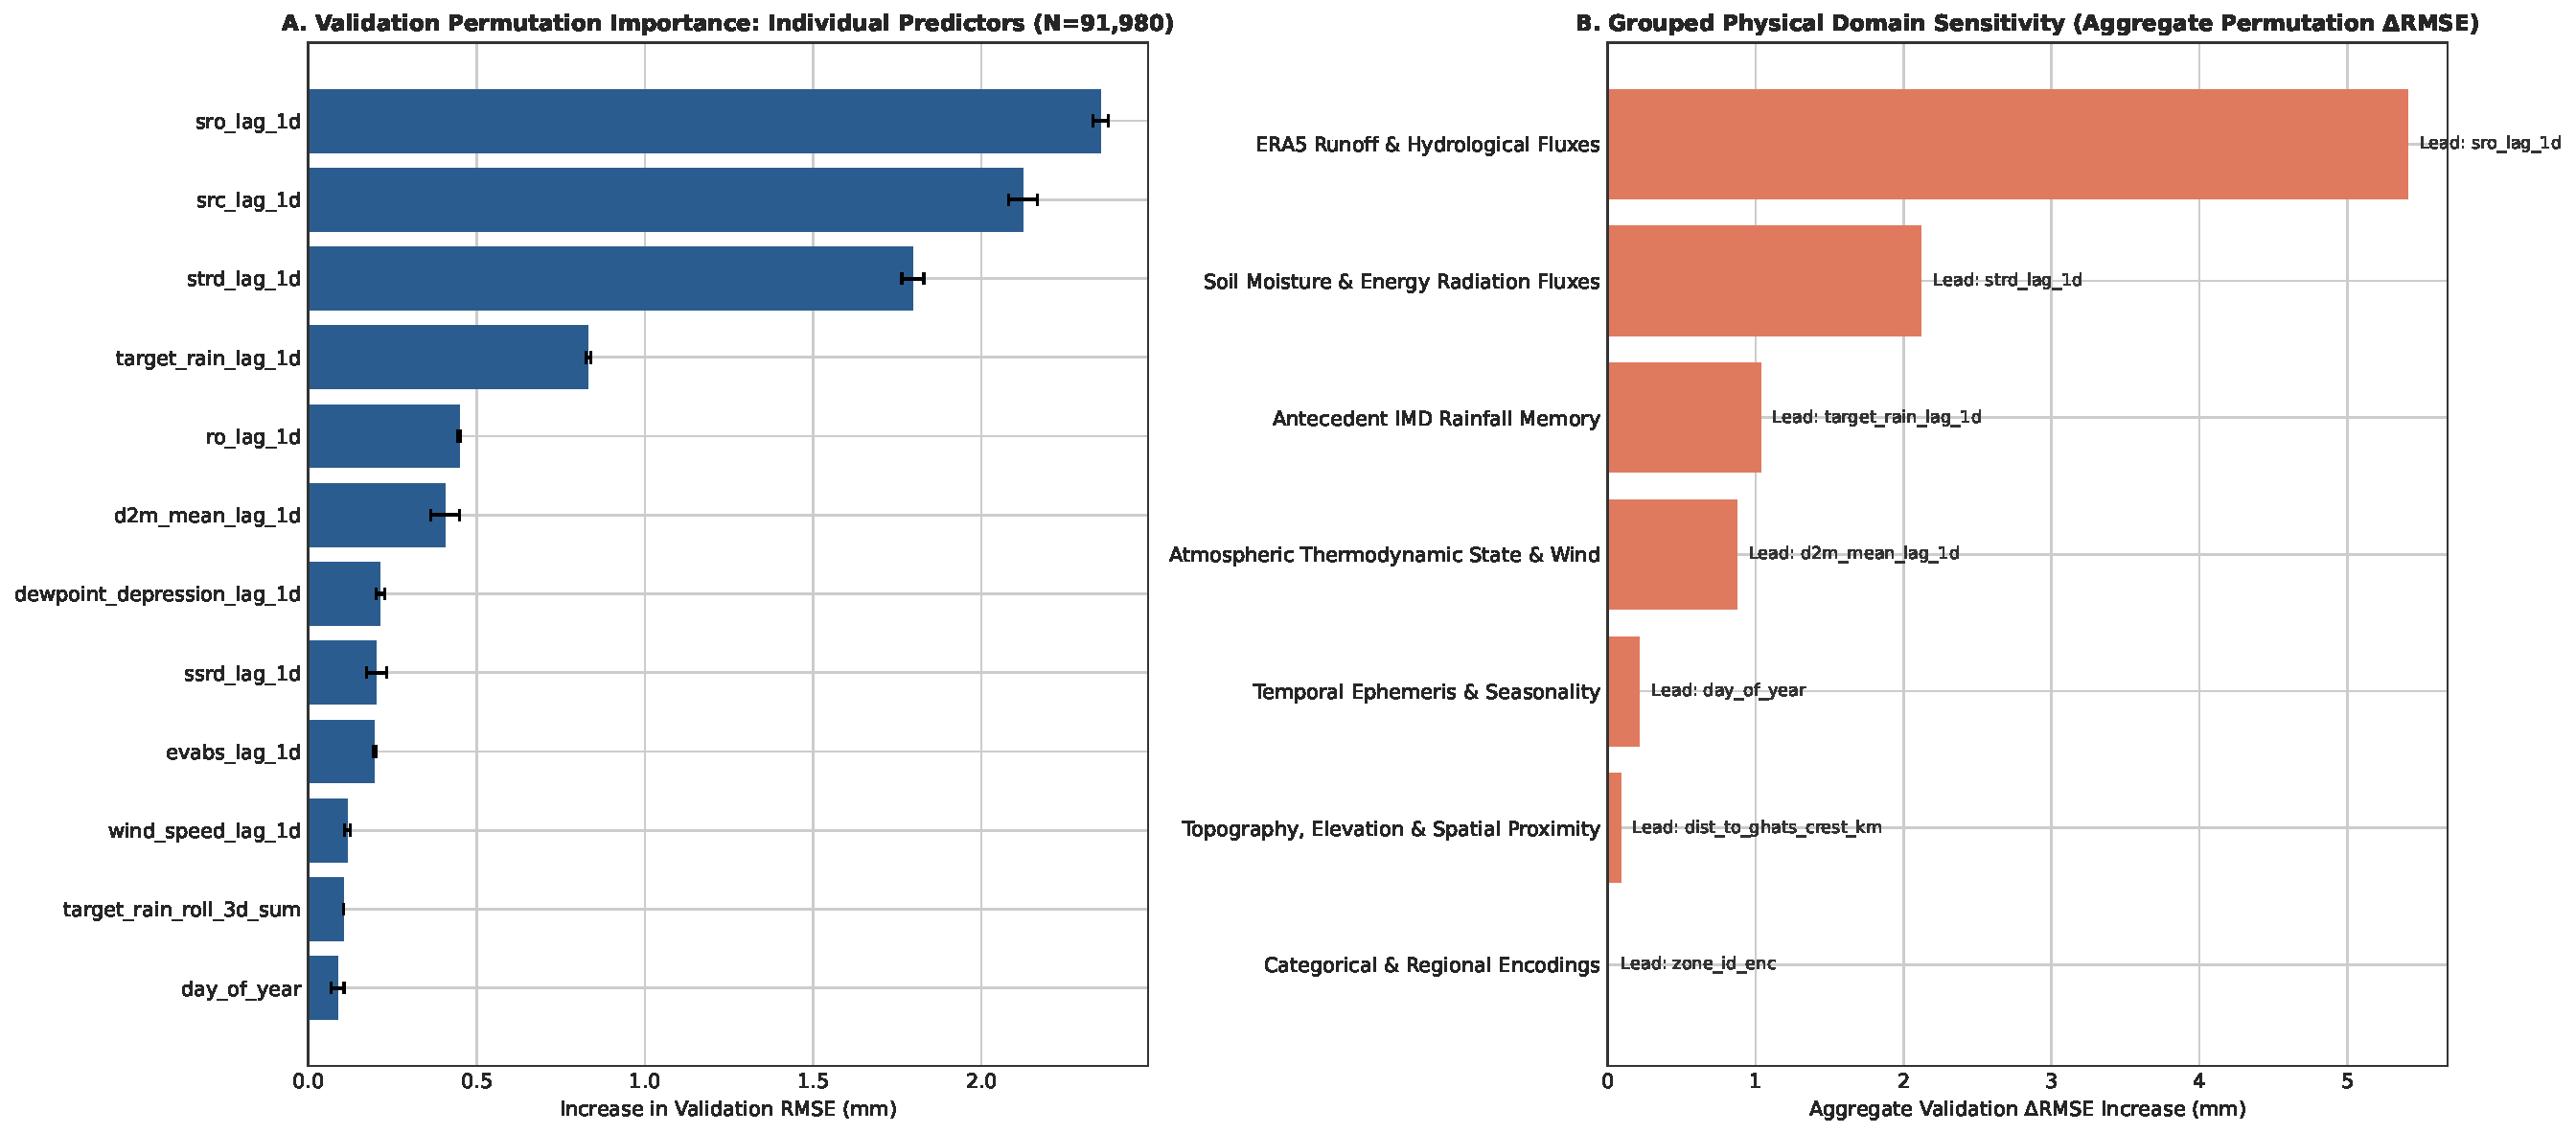
\includegraphics[width=0.85\textwidth]{figures/figure6_feature_interpretation}
\caption{Feature attribution analysis. Panel A shows top 15 predictors ranked by validation permutation RMSE degradation; Panel B shows relative gain contribution by physical predictor domain.}
\label{fig:attribution}
\end{figure}

\begin{table}[htbp]
\centering
\caption{Systematic Feature Ablation Matrix (Validation 2023 and Test 2024--2025)}
\label{tab:ablation}
\resizebox{\textwidth}{!}{
\begin{tabular}{llcr r r r r r r p{4.5cm}}
\toprule
\textbf{Scenario ID} & \textbf{Ablation Description} & \textbf{Features Retained Count} & \textbf{Validation RMSE mm} & \textbf{Validation KGE 2012} & \textbf{Validation Heavy CSI} & \textbf{Test RMSE mm} & \textbf{Test KGE 2012} & \textbf{Test Heavy CSI} & \textbf{$\Delta$ Test RMSE vs Full mm} & \textbf{Scientific Interpretation} \\
\midrule
Scenario A & A All 63 Primary Predictors & 63 & 5.585 & 0.6494 & 0.4098 & 7.4427 & 0.6245 & 0.2868 & 0.0 & Champion full configuration \\
Scenario B & B Without Runoff and Hydrological Fluxes & 55 & 5.7149 & 0.6463 & 0.4129 & 7.6854 & 0.5925 & 0.2721 & 0.2427 & Hydrological land fluxes provide critical moisture saturation proxies \\
Scenario C & C Without Antecedent IMD Rainfall & 51 & 5.7147 & 0.6235 & 0.3316 & 7.5828 & 0.607 & 0.2693 & 0.1401 & Local gauge memory essential for extreme threshold alerting \\
Scenario D & D Without Terrain and Spatial Predictors & 55 & 5.5809 & 0.6479 & 0.4097 & 7.4557 & 0.6252 & 0.2843 & 0.013 & Terrain captures spatial orographic boundaries \\
Scenario E & E Without ERA5 Predictors & 26 & 6.3909 & 0.4181 & 0.2652 & 8.4511 & 0.4833 & 0.1536 & 1.0084 & ERA5 atmospheric predictors provide measurable incremental predictive value \\
Scenario F & F Only Antecedent IMD and Temporal & 18 & 6.4289 & 0.4193 & 0.3043 & 8.5145 & 0.4686 & 0.1456 & 1.0718 & Baseline autoregressive floor \\
\bottomrule
\end{tabular}
}
\end{table}

In the Focal Loss heavy-rain classifier, land-surface runoff fluxes---sub-surface runoff (\texttt{ro\_lag\_1d}, $28.11\%$) and surface runoff (\texttt{sro\_lag\_1d}, $26.41\%$)---together account for $54.52\%$ of total tree split gain. In continuous LightGBM Tweedie regression, surface runoff accounts for $34.61\%$ of gain and skin reservoir content contributes $28.28\%$. In validation permutation importance ($N = 91,980$, 3 seeds), surface runoff ranks first ($+2.3545$\;mm RMSE degradation; $+42.16\%$ increase), followed by skin reservoir storage ($+2.1241$\;mm) and downward longwave flux ($+1.7960$\;mm). Ablation Scenario E demonstrates that withholding ERA5-Land predictors causes test RMSE to jump from $7.4427$\;mm to $8.4511$\;mm ($+1.0084$\;mm), proving their substantial incremental predictive value beyond local gauge memory alone.

\subsection{Regional and Seasonal Disaggregation}
Table~\ref{tab:regional} and Figure~\ref{fig:regional} examine model performance stratified across Karnataka's four meteorological subdivisions and four climatological seasons.

\begin{table}[htbp]
\centering
\caption{Subdivisional and Seasonal Stratified Performance on Test Partition}
\label{tab:regional}
\resizebox{\textwidth}{!}{
\begin{tabular}{lllr r r r r r r r r}
\toprule
\textbf{Stratum Type} & \textbf{Stratum Name} & \textbf{Sample Count} & \textbf{Observed Mean mm} & \textbf{ML RMSE mm} & \textbf{Persistence RMSE mm} & \textbf{Raw ERA5 RMSE mm} & \textbf{ML Mean Bias mm} & \textbf{ML PBias pct} & \textbf{ML Pearson r} & \textbf{ML KGE 2012} & \textbf{ML Heavy CSI 64.5mm} \\
\midrule
Meteorological Subdivision & Coastal Karnataka All 13 cells & 9503 & 13.1855 & 14.9475 & 20.3843 & 19.3674 & -1.3244 & -10.04 & 0.8261 & 0.7407 & 0.362 \\
Meteorological Subdivision & Malnad 35 cells & 25585 & 6.3706 & 9.3018 & 12.7091 & 13.2843 & 0.1661 & 2.61 & 0.8043 & 0.7256 & 0.3441 \\
Meteorological Subdivision & North Interior Karnataka 118 cells & 86258 & 2.3758 & 6.4317 & 9.0913 & 9.5698 & 0.0196 & 0.83 & 0.5274 & 0.3676 & 0.0296 \\
Meteorological Subdivision & South Interior Karnataka 86 cells & 62866 & 2.4364 & 6.0472 & 8.5112 & 8.1312 & 0.0531 & 2.18 & 0.5513 & 0.3723 & 0.0 \\
Meteorological Subdivision & Coastal Fallback Only 3 cells IDs 52 68 125 & 2193 & 13.8286 & 15.5086 & 21.61 & 20.3891 & -0.8294 & -6.0 & 0.828 & 0.7504 & 0.3898 \\
Meteorological Subdivision & Coastal Native Land Only 10 cells & 7310 & 12.9925 & 14.7751 & 20.0019 & 19.0503 & -1.4729 & -11.34 & 0.8258 & 0.7356 & 0.3516 \\
Seasonal Regime & Southwest Monsoon JJAS & 61488 & 7.0215 & 10.1883 & 14.1842 & 14.9381 & 0.1431 & 2.04 & 0.7545 & 0.6451 & 0.3355 \\
Seasonal Regime & Post Monsoon Northeast OND & 46368 & 2.1379 & 6.1093 & 8.829 & 7.9161 & 0.0612 & 2.86 & 0.5628 & 0.3823 & 0.0 \\
Seasonal Regime & Pre Monsoon MAM & 46368 & 2.4463 & 6.6839 & 8.9736 & 8.6417 & -0.3207 & -13.11 & 0.6717 & 0.4859 & 0.093 \\
Seasonal Regime & Winter JF & 29988 & 0.0698 & 0.806 & 1.2303 & 1.2443 & -0.0023 & -3.3 & 0.4881 & 0.3436 & 0.0 \\
\bottomrule
\end{tabular}
}
\end{table}

\begin{figure}[htbp]
\centering
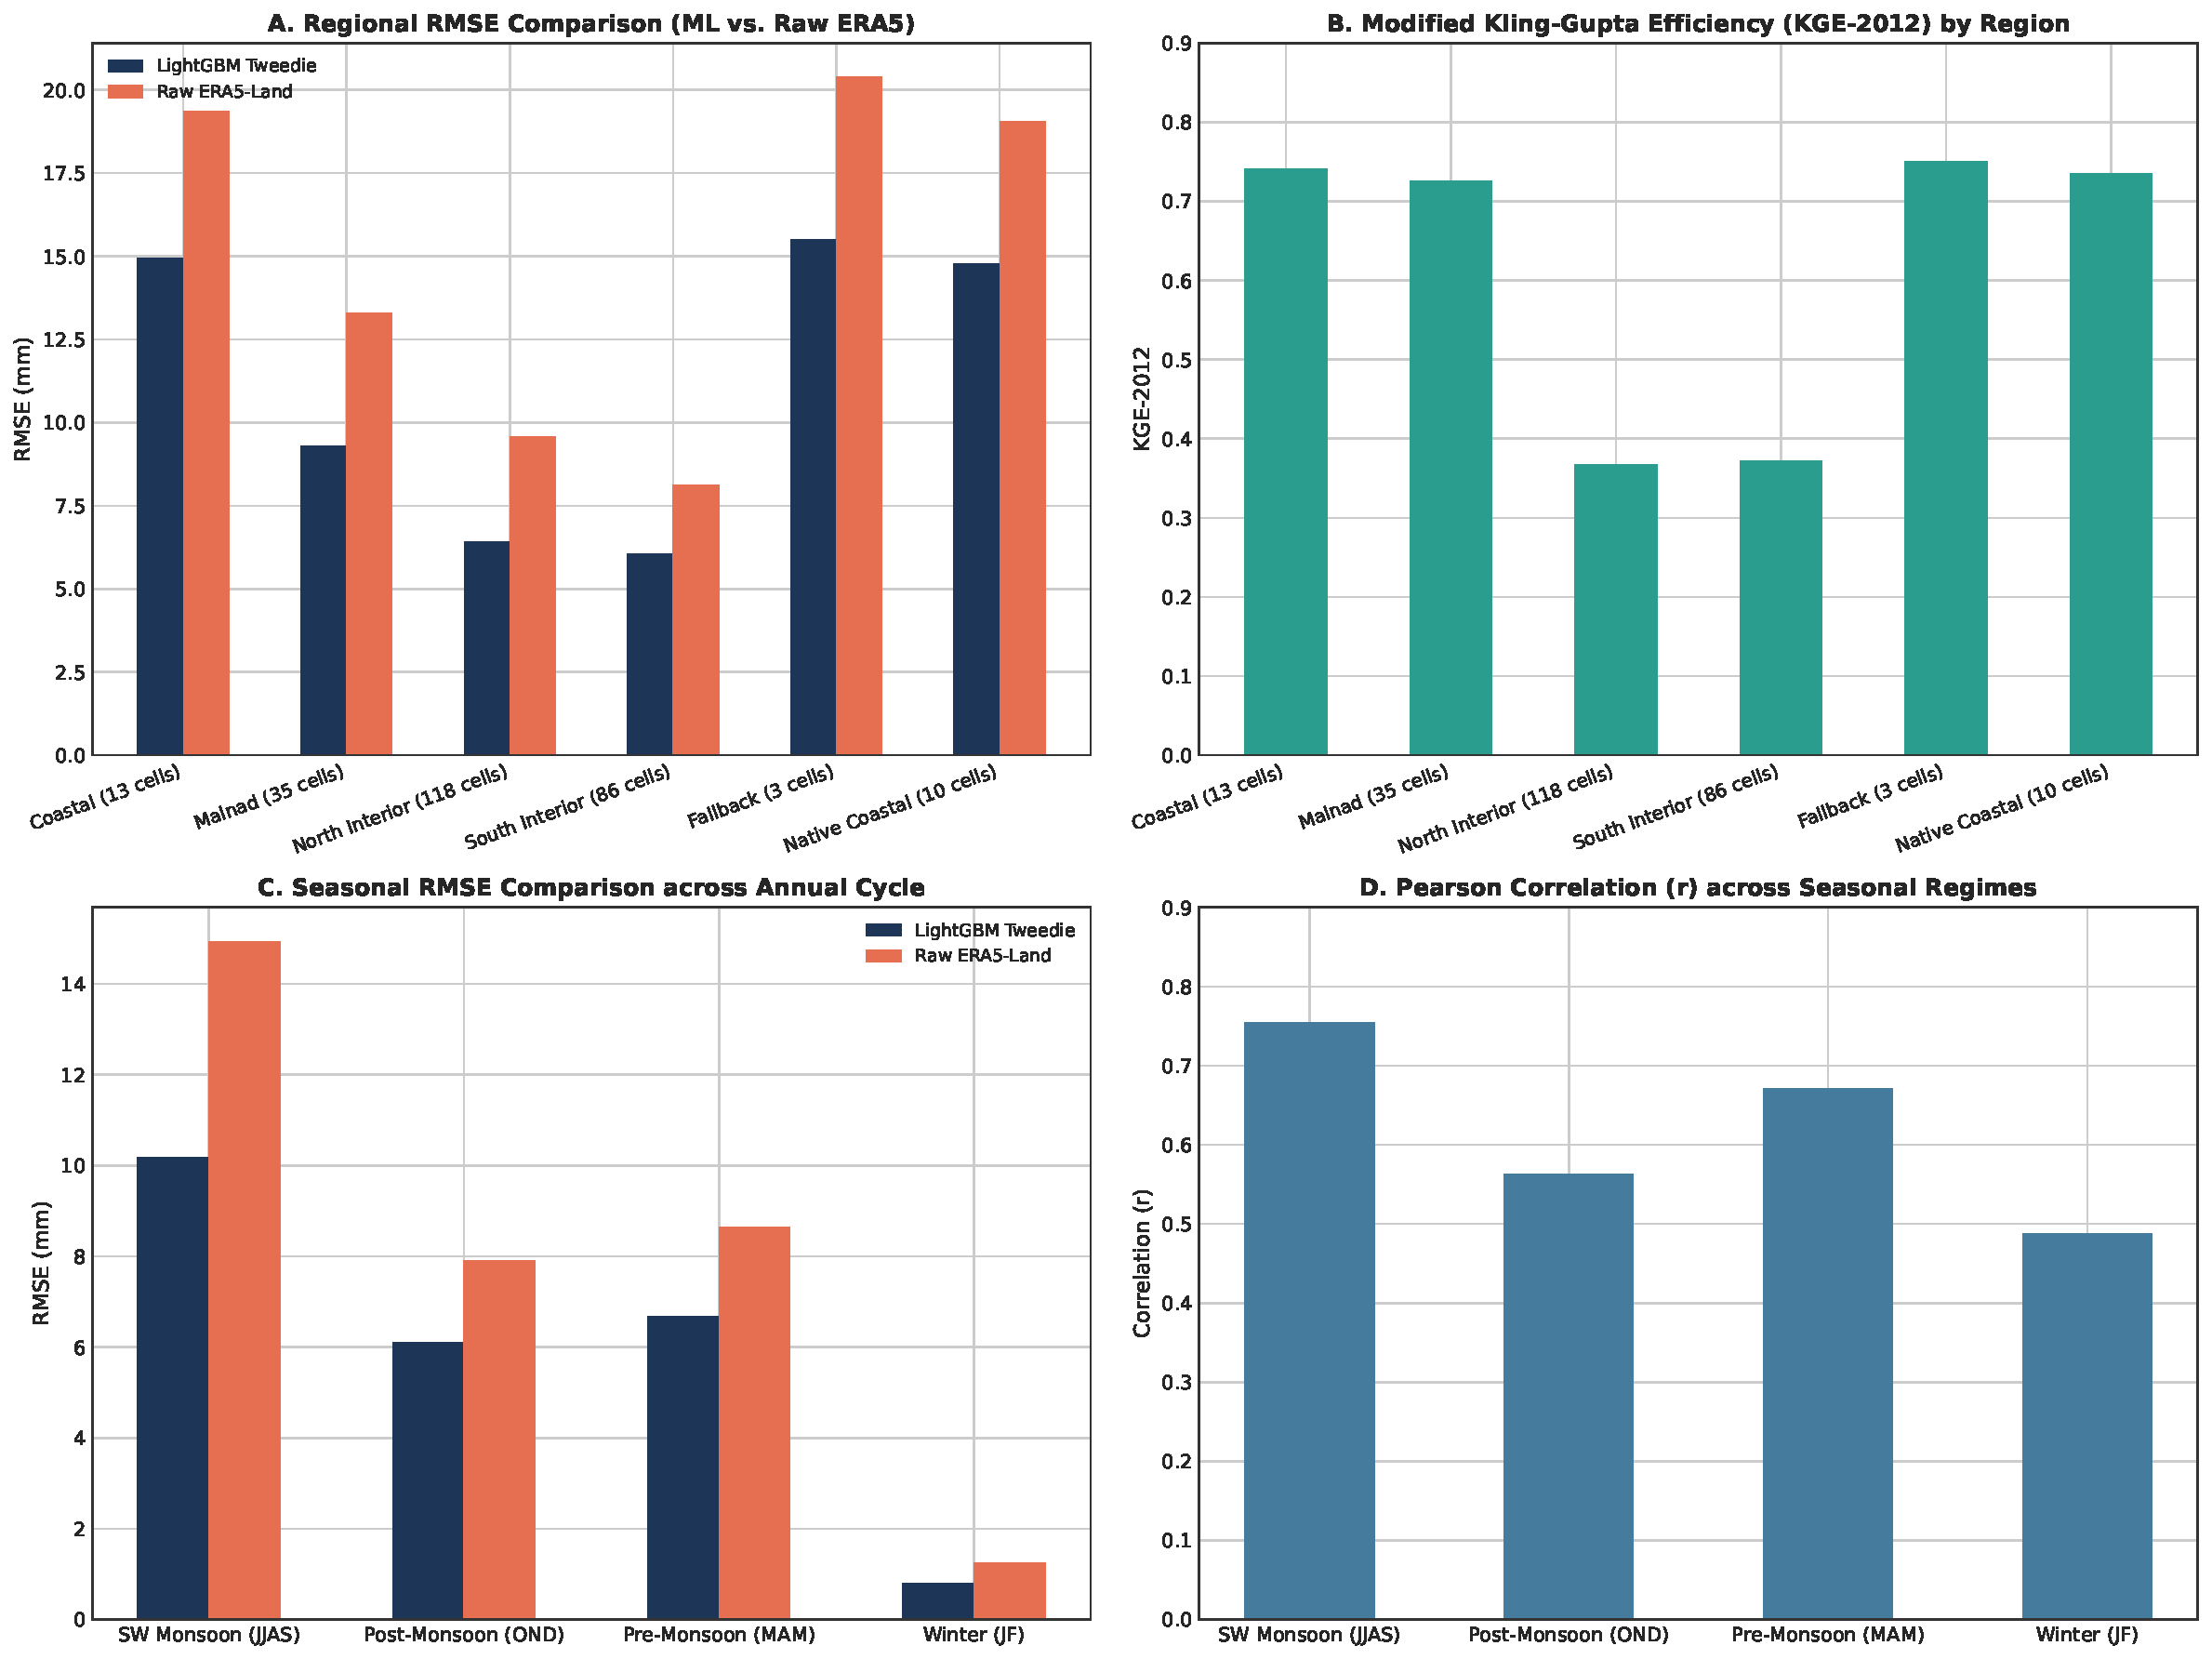
\includegraphics[width=0.88\textwidth]{figures/figure7_regional_seasonal}
\caption{Subdivisional and seasonal hydrometeorological stratification. Panel A shows RMSE and KGE-2012 across subdivisions; Panel B shows seasonal progression across Southwest Monsoon, Post-Monsoon, Pre-Monsoon, and Winter.}
\label{fig:regional}
\end{figure}

The models exhibit stark performance differences across regions. In Coastal Karnataka and Malnad, where rainfall is driven by mechanically forced orographic lifting, the model achieves high correlation ($r = 0.80$--$0.83$) and strong hydrological efficiency ($\text{KGE-2012} = 0.73$--$0.74$). Over the semi-arid interior plains (NIK and SIK), where rainfall is dominated by unorganized, isolated convective thunderstorms, correlation drops to $r \sim 0.53$--$0.55$ and $\text{KGE-2012} \sim 0.37$. For the 3 coastal fallback cells (IDs 52, 68, 125; $N = 2,193$), nearest-inland neighbor substitution yields $\text{RMSE} = 15.51$\;mm and $\text{KGE-2012} = 0.7504$, tracking closely with the 10 native-land coastal cells ($\text{RMSE} = 14.78$\;mm, $\text{KGE-2012} = 0.7356$) and confirming the robustness of the fallback strategy.

\subsection{Temporal Generalisation Across Forward Test Years and Block Bootstrap}
To verify stability across varying climatic regimes, performance was evaluated separately on each forward test year (Table~\ref{tab:annual}):
\begin{itemize}
    \item \textbf{2024 (Leap Year, Active Monsoon):} $N = 92,232$; LightGBM Tweedie achieved $\text{RMSE} = 7.5094$\;mm, $\text{MAE} = 3.0074$\;mm, $\text{Bias} = +0.3442$\;mm ($+10.26\%$), $r = 0.7320$, and $\text{KGE-2012} = 0.5676$.
    \item \textbf{2025 (Subdued Monsoon):} $N = 91,980$; LightGBM Tweedie achieved $\text{RMSE} = 7.3752$\;mm, $\text{MAE} = 2.7909$\;mm, $\text{Bias} = -0.3810$\;mm ($-10.40\%$), $r = 0.7426$, and $\text{KGE-2012} = 0.6541$.
\end{itemize}

\begin{table}[htbp]
\centering
\caption{Annual Out-of-Sample Performance Breakdown: 2024 (Leap Year) vs. 2025}
\label{tab:annual}
\resizebox{\textwidth}{!}{
\begin{tabular}{llr r r r r r r r r r}
\toprule
\textbf{Strata} & \textbf{Model} & \textbf{N} & \textbf{Obs Mean} & \textbf{Pred Mean} & \textbf{MAE mm} & \textbf{RMSE mm} & \textbf{Bias mm} & \textbf{PBias pct} & \textbf{Pearson r} & \textbf{NSE} & \textbf{KGE 2012} \\
\midrule
Year\_2024\_Full & LightGBM\_Tweedie & 92232 & 3.3539 & 3.6981 & 3.0074 & 7.5094 & 0.3442 & 10.26 & 0.732 & 0.5346 & 0.5676 \\
Year\_2024\_Full & CatBoost\_Tweedie & 92232 & 3.3539 & 3.7431 & 3.0289 & 7.5253 & 0.3892 & 11.6 & 0.7309 & 0.5327 & 0.5577 \\
Year\_2024\_Full & Hurdle\_ExpectedValue & 92232 & 3.3539 & 3.7534 & 3.05 & 7.521 & 0.3995 & 11.91 & 0.7311 & 0.5332 & 0.5436 \\
Year\_2024\_Full & Persistence & 92232 & 3.3539 & 3.3539 & 3.6498 & 10.3927 & -0.0 & -0.0 & 0.5543 & 0.1087 & 0.5543 \\
Year\_2024\_Full & Raw\_ERA5 & 92232 & 3.3539 & 4.1579 & 4.1904 & 10.6003 & 0.8041 & 23.97 & 0.4789 & 0.0727 & 0.3527 \\
Year\_2024\_Full & EQM & 92232 & 3.3539 & 3.9681 & 4.2069 & 11.1297 & 0.6142 & 18.31 & 0.493 & -0.0222 & 0.4403 \\
Year\_2025\_Full & LightGBM\_Tweedie & 91980 & 3.6644 & 3.2834 & 2.7909 & 7.3752 & -0.381 & -10.4 & 0.7426 & 0.5493 & 0.6541 \\
Year\_2025\_Full & CatBoost\_Tweedie & 91980 & 3.6644 & 3.3519 & 2.808 & 7.3403 & -0.3125 & -8.53 & 0.7446 & 0.5535 & 0.6689 \\
Year\_2025\_Full & Hurdle\_ExpectedValue & 91980 & 3.6644 & 3.3324 & 2.8096 & 7.3257 & -0.332 & -9.06 & 0.7466 & 0.5553 & 0.6538 \\
Year\_2025\_Full & Persistence & 91980 & 3.6644 & 3.6644 & 3.8522 & 10.3236 & 0.0 & 0.0 & 0.5584 & 0.1168 & 0.5584 \\
Year\_2025\_Full & Raw\_ERA5 & 91980 & 3.6644 & 3.9717 & 4.0926 & 10.3073 & 0.3073 & 8.39 & 0.5038 & 0.1196 & 0.4592 \\
Year\_2025\_Full & EQM & 91980 & 3.6644 & 3.823 & 4.2165 & 11.264 & 0.1586 & 4.33 & 0.4957 & -0.0514 & 0.4938 \\
\bottomrule
\end{tabular}
}
\end{table}

\begin{table}[htbp]
\centering
\caption{Stationary Block Bootstrap Statistical Significance (2,000 Replicates on Test Partition)}
\label{tab:bootstrap}
\resizebox{\textwidth}{!}{
\begin{tabular}{llp{4.5cm}r r r r r c c}
\toprule
\textbf{Model Pair} & \textbf{Block Length Days} & \textbf{Temporal Memory Assumption} & \textbf{Bootstrap Replicates} & \textbf{Mean $\Delta$ RMSE mm} & \textbf{Standard Error mm} & \textbf{CI 95 Low mm} & \textbf{CI 95 High mm} & \textbf{Replicates $\Delta$ ge Zero} & \textbf{Empirical p Value Resolution} \\
\midrule
LightGBM\_Tweedie vs. Persistence & 7 & Synoptic weather persistence (7d) & 2000 & -2.925 & 0.2046 & -3.3241 & -2.5175 & 0 & p $<$ 0.0005 \\
LightGBM\_Tweedie vs. EQM & 7 & Synoptic weather persistence (7d) & 2000 & -3.7542 & 0.3768 & -4.4626 & -3.0039 & 0 & p $<$ 0.0005 \\
LightGBM\_Tweedie vs. Raw\_ERA5 & 7 & Synoptic weather persistence (7d) & 2000 & -3.0109 & 0.3482 & -3.7037 & -2.3735 & 0 & p $<$ 0.0005 \\
CatBoost\_Tweedie vs. Persistence & 7 & Synoptic weather persistence (7d) & 2000 & -2.9337 & 0.2077 & -3.3415 & -2.5276 & 0 & p $<$ 0.0005 \\
CatBoost\_Tweedie vs. EQM & 7 & Synoptic weather persistence (7d) & 2000 & -3.7629 & 0.3848 & -4.4936 & -2.9954 & 0 & p $<$ 0.0005 \\
Hurdle\_ExpectedValue vs. Persistence & 7 & Synoptic weather persistence (7d) & 2000 & -2.9436 & 0.2025 & -3.3413 & -2.5449 & 0 & p $<$ 0.0005 \\
Hurdle\_ExpectedValue vs. EQM & 7 & Synoptic weather persistence (7d) & 2000 & -3.7728 & 0.3824 & -4.4955 & -3.0224 & 0 & p $<$ 0.0005 \\
LightGBM\_Tweedie vs. Persistence & 14 & Bi-weekly intraseasonal / MJO persistence (14d) & 2000 & -2.9298 & 0.2271 & -3.3608 & -2.4729 & 0 & p $<$ 0.0005 \\
LightGBM\_Tweedie vs. EQM & 14 & Bi-weekly intraseasonal / MJO persistence (14d) & 2000 & -3.7645 & 0.4243 & -4.5976 & -2.9587 & 0 & p $<$ 0.0005 \\
LightGBM\_Tweedie vs. Raw\_ERA5 & 14 & Bi-weekly intraseasonal / MJO persistence (14d) & 2000 & -3.0204 & 0.3785 & -3.7669 & -2.3255 & 0 & p $<$ 0.0005 \\
CatBoost\_Tweedie vs. Persistence & 14 & Bi-weekly intraseasonal / MJO persistence (14d) & 2000 & -2.9382 & 0.2322 & -3.38 & -2.4688 & 0 & p $<$ 0.0005 \\
CatBoost\_Tweedie vs. EQM & 14 & Bi-weekly intraseasonal / MJO persistence (14d) & 2000 & -3.7729 & 0.4338 & -4.6235 & -2.955 & 0 & p $<$ 0.0005 \\
Hurdle\_ExpectedValue vs. Persistence & 14 & Bi-weekly intraseasonal / MJO persistence (14d) & 2000 & -2.948 & 0.2293 & -3.3901 & -2.4876 & 0 & p $<$ 0.0005 \\
Hurdle\_ExpectedValue vs. EQM & 14 & Bi-weekly intraseasonal / MJO persistence (14d) & 2000 & -3.7827 & 0.4309 & -4.6238 & -2.963 & 0 & p $<$ 0.0005 \\
\bottomrule
\end{tabular}
}
\end{table}

\begin{figure}[htbp]
\centering
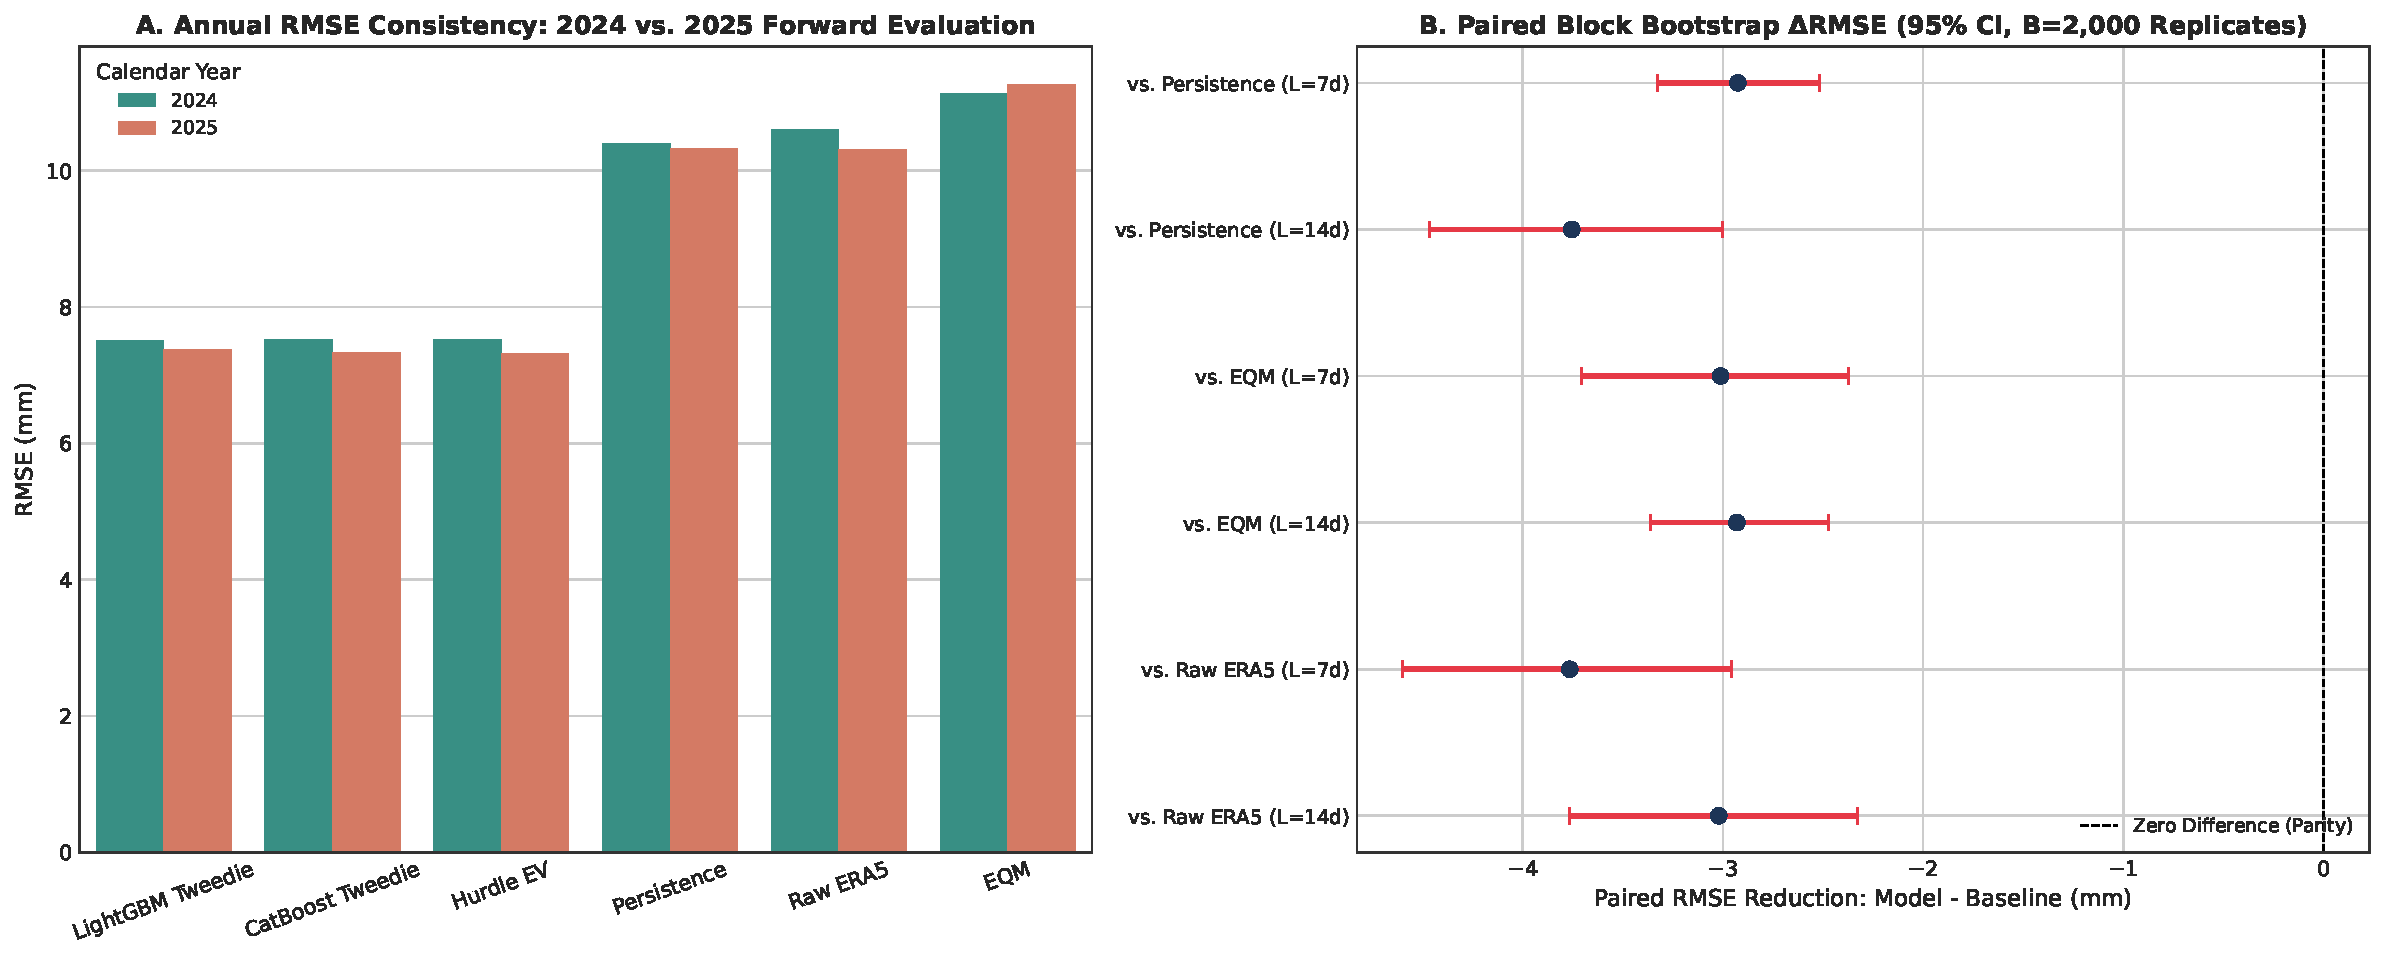
\includegraphics[width=0.88\textwidth]{figures/figure8_temporal_robustness}
\caption{Temporal robustness and block bootstrap confidence intervals. Panel A shows annual RMSE consistency bar comparison across 2024 and 2025 forward evaluation years; Panel B shows paired block bootstrap 95\% confidence interval error bars ($B = 2,000$ replicates, empirical resolution $p < 0.0005$) for $L=7\text{d}$ and $L=14\text{d}$ block lengths.}
\label{fig:robustness}
\end{figure}

Across all 2,000 paired stationary block bootstrap resamples under both 7-day and 14-day block lengths (Table~\ref{tab:bootstrap} and Fig.~\ref{fig:robustness}), exactly zero replicates produced $\Delta \text{RMSE} \ge 0$. This provides rigorous empirical evidence of statistically significant superiority over autoregressive Persistence and raw ERA5-Land ($p < 0.0005$).

\subsection{Rainfall Intensity Limitations and Extreme Quantile Shrinkage}
Table~\ref{tab:intensity} and Figure~\ref{fig:extremes} provide an audit across all seven official IMD rainfall intensity categories.

\begin{table}[htbp]
\centering
\caption{Rainfall Intensity Error Profiles and Extreme Quantile Shrinkage (Test Set; $N = 184,212$)}
\label{tab:intensity}
\resizebox{\textwidth}{!}{
\begin{tabular}{lr r r r r r r r r r r p{4cm}}
\toprule
\textbf{IMD Rainfall Intensity Category} & \textbf{Sample Count} & \textbf{Percent Total Test Data} & \textbf{Observed Mean mm} & \textbf{Observed Std mm} & \textbf{Predicted Mean mm} & \textbf{Predicted Std mm} & \textbf{MAE mm} & \textbf{RMSE mm} & \textbf{Mean Bias mm} & \textbf{Percentage Bias pct} & \textbf{Percent Underestimated} & \textbf{Structural Limitation Note} \\
\midrule
No Rain ($<$0.1 mm) & 119669 & 64.96 & 0.0 & 0.0 & 0.77 & 1.96 & 0.77 & 2.1 & 0.77 & Undefined\textsuperscript{*} & 0.0 & Near-zero background drizzle inflation \\
Very Light (0.1--2.4 mm) & 26590 & 14.43 & 0.96 & 0.69 & 4.04 & 4.04 & 3.29 & 5.05 & 3.08 & 319.1 & 16.9 & Overestimation due to exponential link penalty \\
Light (2.5--15.5 mm) & 25854 & 14.03 & 7.03 & 3.6 & 7.46 & 6.53 & 4.67 & 6.58 & 0.43 & 6.1 & 53.8 & Optimal continuous calibration sweet spot \\
Moderate (15.6--64.4 mm) & 10832 & 5.88 & 29.81 & 12.29 & 17.22 & 15.23 & 16.55 & 20.21 & -12.59 & -42.2 & 83.5 & Progressive underestimation onset \\
Heavy (64.5--115.5 mm) & 1067 & 0.58 & 81.68 & 13.12 & 46.98 & 28.89 & 37.58 & 44.39 & -34.71 & -42.5 & 88.6 & Severe extreme quantile shrinkage (conditional expectation cap) \\
Very Heavy (115.6--204.4 mm) & 192 & 0.1 & 141.52 & 20.68 & 71.53 & 27.63 & 70.0 & 77.72 & -70.0 & -49.5 & 100.0 & Severe extreme quantile shrinkage (conditional expectation cap) \\
Extremely Heavy ($\ge$204.5 mm) & 8 & 0.0043 & 225.02 & 18.7 & 73.66 & 27.99 & 151.36 & 154.76 & -151.36 & -67.3 & 100.0 & Severe extreme quantile shrinkage (conditional expectation cap) \\
\bottomrule
\end{tabular}
}
\end{table}

\begin{figure}[htbp]
\centering
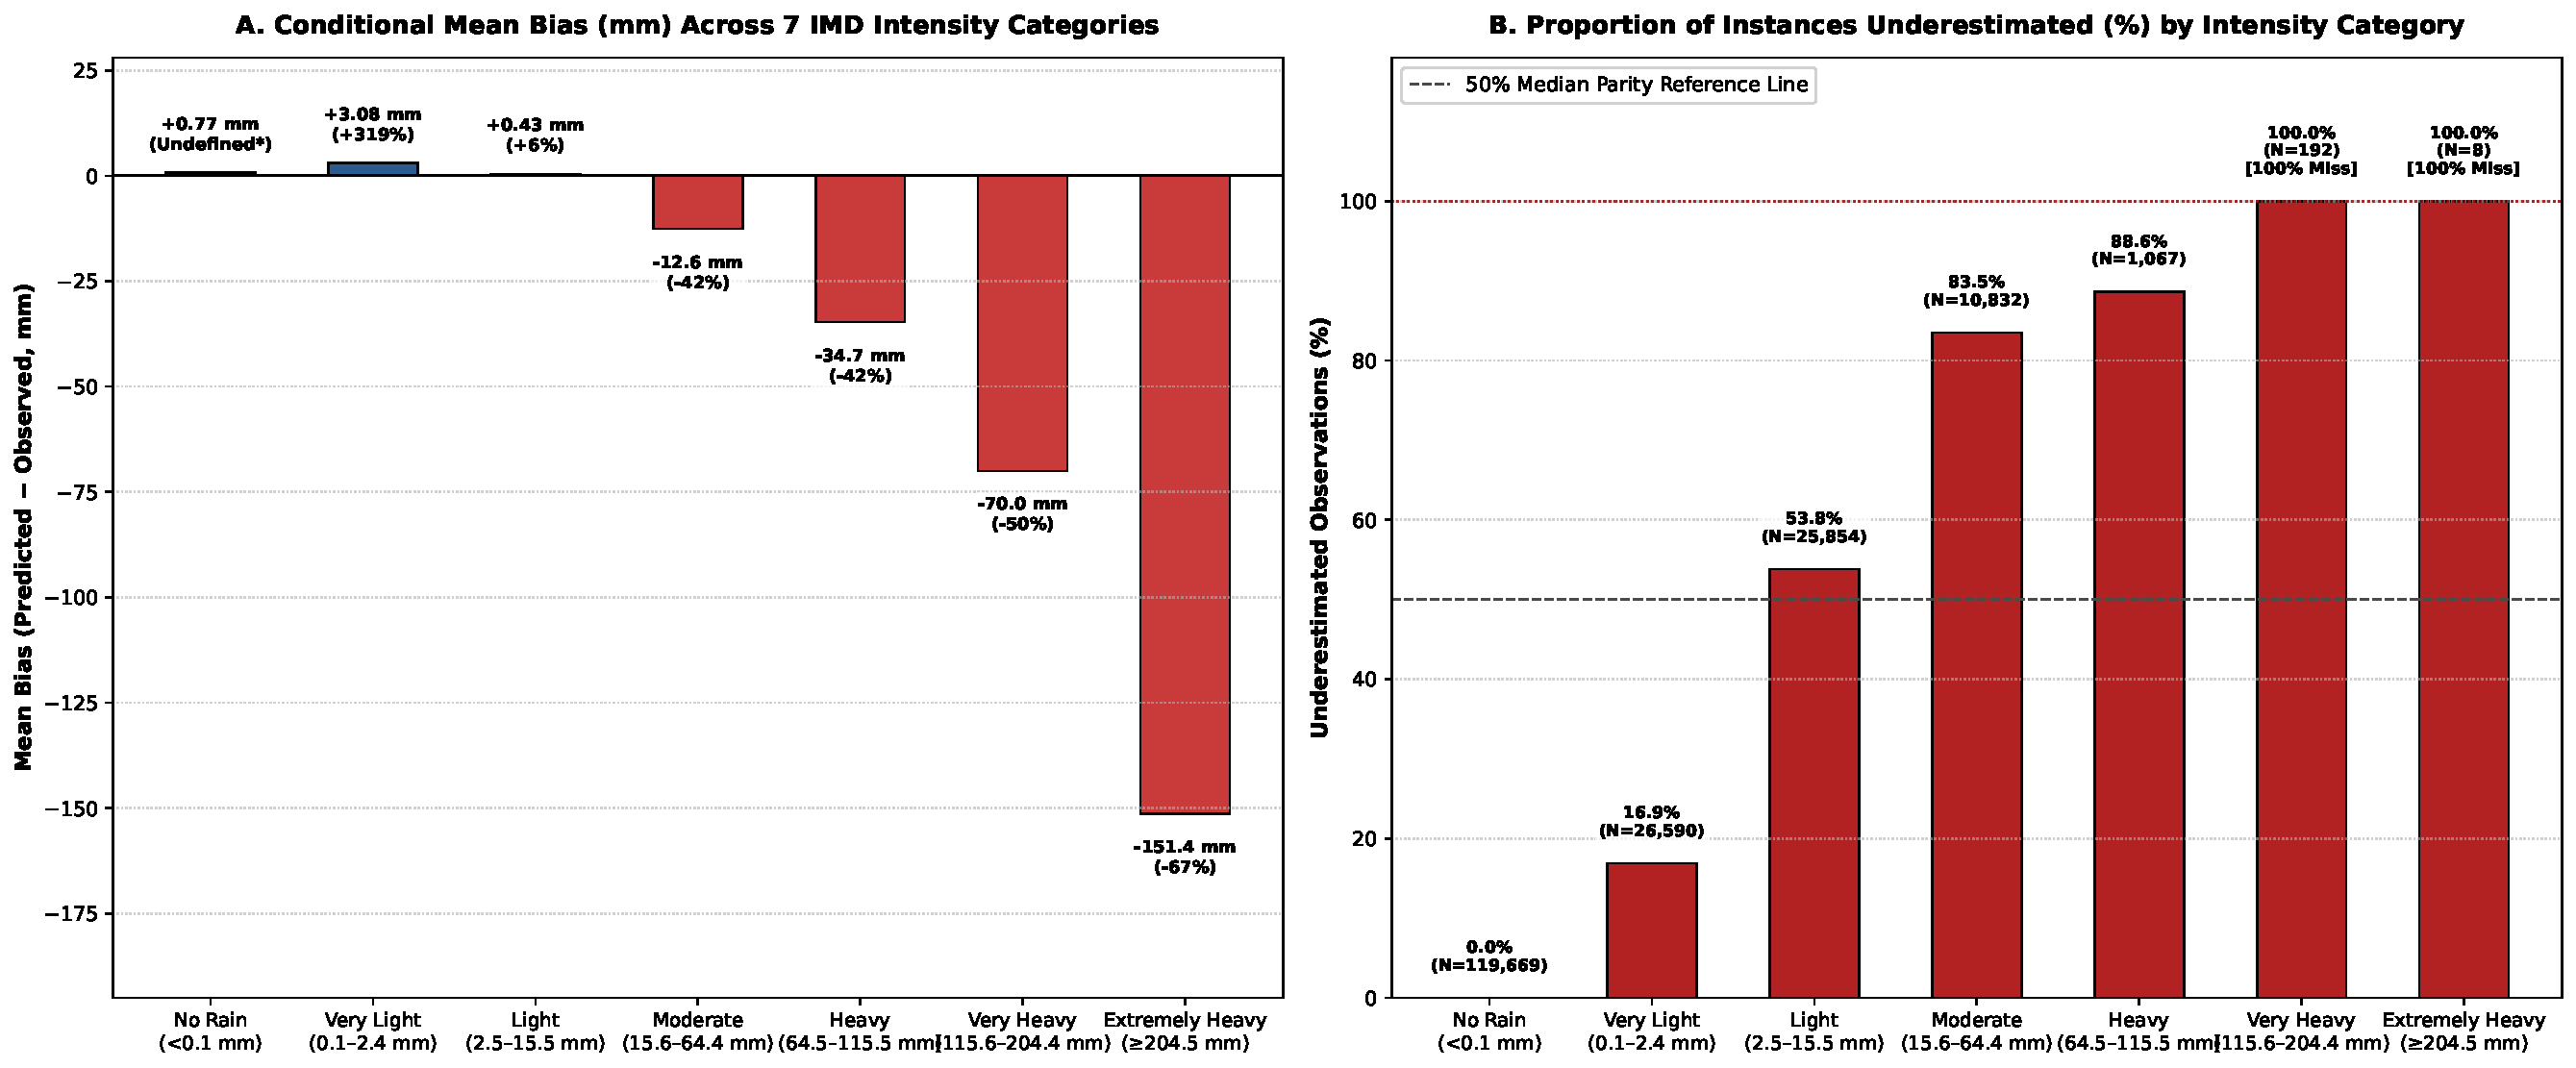
\includegraphics[width=0.88\textwidth]{figures/figure9_extreme_rainfall_errors}
\caption{Rainfall intensity error profiles and quantile shrinkage. Panel A shows Mean Bias (mm) and Percentage Bias (\%) across the 7 IMD categories; Panel B shows underestimation frequency (\%) and sample counts.}
\label{fig:extremes}
\end{figure}

A critical structural boundary is documented: \textbf{continuous models underestimate $100.0\%$ of events exceeding 115.6~mm/day} (200 test events, including 192 Very Heavy and 8 Extremely Heavy days). Model predictions plateau at approximately $70$--$90$\;mm despite observed local gauge extremes reaching $286.0$\;mm. Additionally, on true dry days ($<0.1$\;mm; $64.96\%$ of test data), the model introduces a slight background drizzle inflation ($+0.77$\;mm mean bias).

\subsection{Comprehensive Discussion}

\subsubsection{Hydrological Memory: Surface Runoff as Soil Saturation Proxy}
The finding that antecedent reanalysis runoff fluxes dominate feature importance ($54.52\%$ of classification gain) reveals a key physical mechanism. ERA5-Land runoff is a simulated flux generated by the HTESSEL land-surface scheme when topsoil layers reach moisture saturation or rainfall exceeds infiltration capacity. Because soil moisture has substantial temporal inertia in tropical soils, antecedent runoff serves as an integrated physical proxy for basin-wide saturation, filtering out transient cloud anomalies and indicating high antecedent moisture convergence.

\subsubsection{The Conditional Mean Ceiling and Disaster-Risk Alerting Limitations}
The complete underestimation of rainfall exceeding 115.6~mm/day is not an idiosyncratic bug but a mathematical consequence of minimizing squared-error and deviance loss functions over highly skewed distributions. Because extreme events comprise less than $0.1\%$ of the dataset, optimal conditional expectation estimation shrinks predictions toward the bulk conditional mean. For operational flood warning, continuous regression must be decoupled from extreme hazard alerting.

\subsubsection{Orographic Trade-offs and Spatial Bias Dissociation}
The dichotomy between orographic zones ($r \ge 0.80$) and interior plains ($r \sim 0.53$) reflects physical scale limits. Orographic lifting along the Western Ghats is governed by synoptic-scale windward moisture convergence that 0.1$^\circ$ reanalysis resolves well. In contrast, interior rainfall is driven by meso-convective thunderstorms with spatial scales smaller than reanalysis grid resolution, setting an intrinsic predictability ceiling for coarse reanalysis predictors.

\subsubsection{Prerequisites for Operational Deployment}
Because ERA5-Land operates with a 2- to 3-month public release latency, this framework represents a diagnostic retrospective reconstruction pipeline. Operational real-time deployment would require:
\begin{enumerate}
    \item Replacing retrospective reanalysis with real-time operational NWP forecasts (such as ECMWF IFS or IMD WRF).
    \item Ingesting real-time Doppler weather radar (DWR) reflectivity profiles.
    \item Calibrating extreme-value loss functions (e.g., threshold-weighted CRPS or generalized Pareto tails).
\end{enumerate}

\subsection{Key Limitations of the Study}
\begin{enumerate}
    \item \textbf{Retrospective Scope:} Reanalysis data latency precludes live, same-day flood nowcasting.
    \item \textbf{No Spatial Generalisation:} Models were evaluated across the same 252 grid cells across time; performance in completely ungauged basins was not tested.
    \item \textbf{Severe Extreme Event Shrinkage:} 100\% underestimation of rainfall exceeding 115.6~mm/day due to conditional mean plateauing.
    \item \textbf{Focal Loss Miss Rate:} Missing 53.04\% of heavy events ($\ge 64.5$\;mm) prevents its use as a standalone operational warning system.
    \item \textbf{Dry-Day Drizzle Inflation:} A background drizzle artifact of $+0.77$\;mm on dry days.
\end{enumerate}

\newpage
\section{Conclusion}

\subsection{Synthesis of Findings}
In this mini project, we formulated, implemented, and rigorously verified a machine-learning framework for daily retrospective rainfall reconstruction across Karnataka State using 7 years of ERA5-Land reanalysis and IMD gridded observations (2019--2025; $N = 640,836$). Operating under strict 24-hour causal latency gating ($T_{\text{issue}} = \text{03:00 UTC day } t-1$), our findings demonstrate:
\begin{enumerate}
    \item Machine-learning models achieve substantial, statistically significant improvements over classical downscaling, reducing RMSE by $\sim$28.9\% relative to raw ERA5-Land and $\sim$28.3\% relative to persistence ($p < 0.0005$).
    \item The top architectures exhibit complementary multi-criteria trade-offs: Hurdle Expected Value delivers lowest RMSE ($7.4241$\;mm) and highest NSE ($0.5443$); CatBoost Tweedie attains highest KGE-2012 ($0.6261$); and LightGBM Tweedie yields lowest MAE ($2.8993$\;mm) and lowest bias ($-0.0179$\;mm).
    \item Antecedent land-surface runoff fluxes act as vital physical proxies for basin soil saturation, accounting for over $54\%$ of tree split gain in heavy-rain classification.
    \item Severe extreme-quantile shrinkage restricts continuous models from capturing convective storms $>115.6$\;mm/day, demonstrating the necessity of separating continuous water-balance modeling from extreme hazard detection.
\end{enumerate}

\subsection{Agronomic and Water Resources Management Implications}
For agricultural planning across Karnataka, these models provide reliable historical daily water-budget reconstructions, enabling accurate monitoring of crop water availability, agricultural drought severity indexing, and retrospective crop insurance claim verification. In rain-shadow districts of North Interior Karnataka, the framework offers valuable quantitative insights into soil moisture dynamics and monsoon dry-spell duration.

\subsection{Future Research Directions}
Future work will focus on:
\begin{itemize}
    \item Ingesting high-resolution Doppler Weather Radar (DWR) telemetry and INSAT-3D/3DR geostationary satellite infrared imagery.
    \item Exploring spatiotemporal deep-learning architectures, including Convolutional LSTMs and Graph Neural Networks (GNNs), to capture cross-basin advection dynamics.
    \item Formulating asymmetric extreme-value loss functions based on Generalized Extreme Value (GEV) distributions to lift the conditional mean ceiling during extreme cloudbursts.
\end{itemize}

\newpage
\settocbibname{References}
\bibliography{Myreferences}

\end{document}
